\documentclass{article}
\usepackage[utf8]{inputenc}
\usepackage{geometry}
\geometry{top=80px, bottom=80px, left=70px, right=70px}
\usepackage{amsmath}
\usepackage{amssymb}
\usepackage{algorithm}
\usepackage{algorithmic}
\usepackage{indentfirst}
\usepackage{setspace}
\onehalfspacing
\usepackage{url}
\usepackage{hyperref}
\newcommand\tab[1][1cm]{\hspace*{#1}}
\usepackage{listings}
\usepackage{xcolor}
\usepackage{changepage}
\usepackage{graphicx}
\usepackage[pages=some]{background}
\usepackage{array}
\usepackage{dirtree}
\usepackage{subfig}

\newcommand\myicon[1]{{\color{#1}\rule{2ex}{2ex}}}
\newcommand{\myfolder}[2]{\myicon{#1}\ {#2}}

\renewcommand{\baselinestretch}{1.15}

\hypersetup{
    colorlinks=true,
    linkcolor=black,
    filecolor=magenta,
    urlcolor=blue,
}

\lstset
{
    breaklines=true,
    breakatwhitespace=true,
    frame=single,
    columns=fullflexible,
    basicstyle=\ttfamily,
    showstringspaces=false,
    %numbers=left,
    %stepnumber=1,
    %numbersep=8pt,
}

\backgroundsetup{
scale=1,
color=black,
opacity=0.05,
angle=10,
position={12cm,-22cm},
contents={%
  
\includegraphics[height=20cm,width=20cm,keepaspectratio]{images/sceau.jpg}
  }%
}

%\newcommand\tab[1][1cm]{\hspace*{#1}}
\newcommand\bld[1]{\textbf{#1}}
\newcommand\ita[1]{\textit{#1}}
\newcommand\pcw[1]{\texttt{#1}}

\begin{document}
\begin{titlepage}
    \begin{center}
        \BgThispage
        \vspace*{1cm}
        
        
        \huge
        \textbf{Data Mining}
        \vspace{0.25cm}
        
        \LARGE
        \textbf{INFO-H423}
        
        \vspace{0.5cm}
        \LARGE
        {Hack my Ride}
        
        
        \vspace{3.5cm}
        
        \textbf{BAKKALI Yahya (000445166) \\}
        \textbf{FALLAHI Amirmohammad (000460073) \\}
        \textbf{HAUWAERT Maxime (000461714) \\}
        \textbf{NIZERY Damien (000544100) \\}
    
        \vspace{2.5cm}
        \textit{December 2021 \\}
        \vspace{0.5cm}
        \textsc{Université Libre de Bruxelles (ULB)}
        
        
    \end{center}
\end{titlepage}

\tableofcontents
%\thispagestyle{empty}
\newpage
%\setcounter{page}{1}
\setlength{\parskip}{1em}

\section{Introduction}

Public transport is a vital part of nowadays societies. In addition to allowing people to travel from a location to another location, it can really be useful to find solutions to some of today's environmental problems. If a public transport company provides good services, people will give it some credit, so that in addition to increasing its profit, urban traffic, energy consumption and air pollution can be decreased.

A profound study and good analysis of public transport companies' data and statistics can help the managers and the experts of these companies to provide a more accurate schedule, and it can also be useful for the users, to organize their daily program. In this project, data from Brussels' intercommunal transport company, \textbf{STIB/MIVB}\footnote{"Société des Transports Intercommunaux de Bruxelles" in French or "Maatschappij voor het Intercommunaal Vervoer te Brussel" in Dutch}, has been analyzed. The following analyses have been performed on data ranging from the \textit{3\textsuperscript{rd} September 2021} to the \textit{23\textsuperscript{rd} September 2021}:
\begin{itemize}
    \item Vehicle's speed variation over time.
    \item Vehicle's delays at the different stops.
    \item Prediction on the vehicles' arrival time at a specific stop.
    \item Guessing of the transport mode of a given trajectory over STIB network.
    \item Reachable places within a time interval.
\end{itemize}

In this report, data exploration, data processing, implementation evaluation and also results of each task are explained in detail.


\section{Data preparation}

\subsection{Steps}
\subsubsection{JSON to CSV}

The dataset is composed of several JSON files which contain the location of all vehicles approximately every 30 seconds over a period of 3 weeks.

Analyzing the JSON files is far from easy with the tools at our disposal, and so the first step was to convert the JSON files to CSV files. The way the conversion was performed can be found below:

\begin{tabular}{p{6cm}|p{8cm}}

\hspace{2cm} Before & \hspace{5cm} After \\

\begin{lstlisting}[frame=none, escapechar=!]

{"data":[{
  !\colorbox{green}{"time"}!:"1632409236387",
  "responses":[
     {"lines": [
       {!\colorbox{green}{"lineId"}!: "1",
       "vehiclePositions": [
	    {!\colorbox{green}{"directionId"}!: "8161",
            !\colorbox{green}{"distanceFromPoint"}!: 1,
            !\colorbox{green}{"pointId"}!: "8122"}, ...]}, "lineId": ...]
       },{"lines":...}
   ],}, {...}, ... ]}

\end{lstlisting}

&
\vspace{2cm}
\begin{center}
\begin{tabular}{|c|c|c|c|c|} 
 \hline
 \colorbox{green}{time} & \colorbox{green}{lineId} &\colorbox{green}{directionId} & \colorbox{green}{distanceFromPoint} &  \colorbox{green}{pointId}\\ [0.5ex] 
 \hline\hline
 1632409236387 & 1 & 8161 & 1 & 8122 \\ 
 \hline
 ... & ... & ... & ... & ... \\
 \hline
 ... & ... & ... & ... & ... \\
 \hline
 ... & ... & ... & ... & ... \\
 \hline
\end{tabular}
\end{center}

\end{tabular}

\subsubsection{Lines information}

The data, generated in CSV format, was not sufficient to begin the analyses. The next step was to link the data to other information stored in other dataset files.

The information about the lines in the GTFS files were not easy to handle and were lacking some useful data, such as the distance between the different stops of the lines.

To this purpose, the Esri Shape file describing the map stops of the \textbf{STIB/MIVB} network was used. First, it was loaded using QGIS tools and then saved as a CSV file containing its base attribute values and a new distance field. This new field was computed for each stop and represents the distance to the start point of the line. The following formula was used to compute this distance in QGIS.

\begin{lstlisting}
line_locate_point(geometry:=geometry(get_feature('Lines','LIGNE',"Code_Ligne")),point:=$geometry)
\end{lstlisting}

\subsection{Main challenges}

\subsubsection{Incoherent stop IDs} 
The stop IDs given in the positions files do not seem to correspond directly to the stop IDs in the GTFS files. Some stops present in the different lines have an ID which include a letter. By performing a quick search on the positions files, none of these stops showed up, which led this issue to be investigated further.

First, two sets, \textbf{realStops} and \textbf{posStops} are created and filled the extracted stop IDs from the GTFS files, and from the positions file, respectively.

\paragraph{Direct matching} Matching directly the stop IDs of \textbf{posStops} with the stops of \textbf{realStops}

By removing these stop IDs, there are $21\%$ of the stops that have not been successfully found.

\paragraph{Leading zeroes} Adding leading zeroes to the stop IDs of \textbf{posStops} to get a four characters ID.

By removing these stop IDs, there are still $19\%$ of the stops that are still not found.

There are not any stops in \textbf{realStops} which have the same ID without leading zeroes.

\paragraph{Letter} Matching the stops of \textbf{posStops} with the stops of \textbf{realStops}, which are taken without the possible letter in their IDs.

By deleting these stop IDs, there are finally $4\%$ of the stops that cannot be found.

There are stops in \textbf{realStops} which have the same ID with different letters, but they belong to different lines, which is not a problem as the vehicle positions have a specific line.

The stops that are left in \textbf{posStops} are stops that do not correspond to any of the stops of \textbf{realStops}. Following the STIB documentation, these stops are \textit{technical} stops and must be ignored.

\paragraph{Result}

The stop IDs contained in the positions files underwent a certain trim function. To retrieve their real IDs, the verifications specified above are used. When an ID is still not found even after these verifications, it is treated as a \textit{technical} stops, thus, ignored.


\subsubsection{Variance}

Another useful information to add to the positions files is the variance. Indeed, the variance shows in which direction the vehicles, in a line, go, which is important to get the order of the stops the vehicles should follow.

The way this information is computed by taking the two orders of the stops ID of a line, the first and second variance. Then, iterating backwards in the two lists at the same time and returning the first variance which matched the direction ID.

This works because normally there are no stops IDs in one variance that are also present in the other. There is only one exception, as certain lines have their last stop ID of a variance equal to the first stop ID of the other variance. The computation explained above takes into account this exception.


\subsubsection{Vehicle ID}

One of the most important yet difficult to get information is the vehicle ID. It is the ability of tracking a vehicle through different positions at different times.

It has been chosen to link the different positions to the nearest vehicles available.
In other words, all the positions of a specific line and variance at a certain time $T$ are taken and ordered by their distance from the start of the line. Then, all of these positions are tried to be associated with the available vehicles which have their last position the nearest from it but located before it on the line. It is assumed that a vehicle cannot go backwards. The notion of availability of a vehicle is defined such that a position with a time $T$ cannot be linked to a vehicle which its last position has the same $T$. The positions which could not have been associated with another vehicle have been linked to new vehicles.

\begin{figure}[H]%
    \centering
    \subfloat[\centering T]{{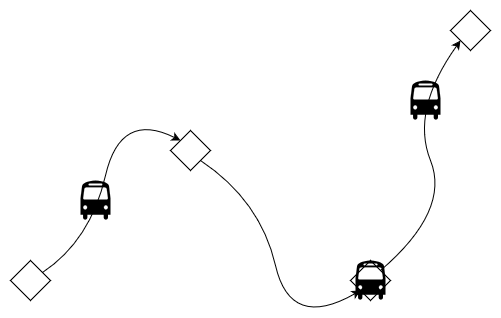
\includegraphics[width=7cm]{images/VehicleIDT.png}  }}%
    \qquad
    \subfloat[\centering T+1]{{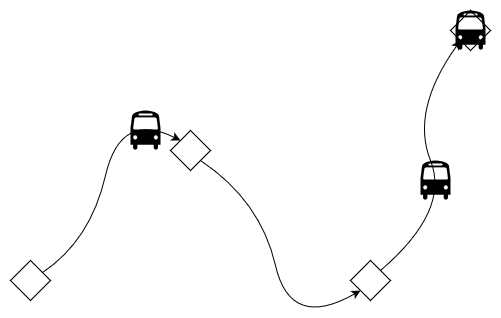
\includegraphics[width=7cm]{images/VehicleIDT1.png} }}%
    \caption{Raw vehicles positions}%
\end{figure}

\begin{figure}[H]%
    \centering
    \subfloat[\centering T]{{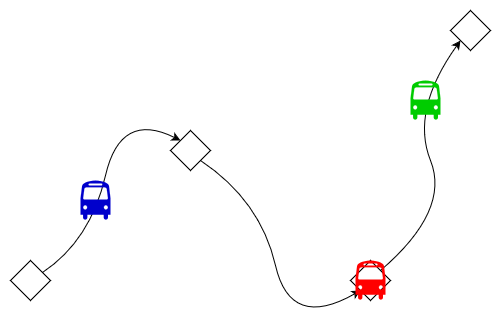
\includegraphics[width=7cm]{images/VehicleIDTColor.png}  }}%
    \qquad
    \subfloat[\centering T+1]{{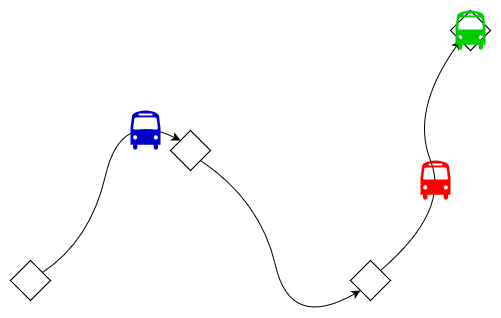
\includegraphics[width=7cm]{images/VehicleIDT1Color.png} }}%
    \caption{Labelized vehicles positions}%
\end{figure}


For this information to be able to be computed as accurately as possible, some additional assumptions had to be made:

\begin{itemize}
    \item The maximum speed a vehicle can have is $100\ km/h$.
    \item The vehicle cannot have the time of two consecutive positions separated by more than two minutes.
\end{itemize}


\subsection{Cleansing}
With all the new information computed and extracted, some erroneous or incoherent pieces of data can be detected and thus removed.

\begin{itemize}
    \item Some positions have a direction ID which is not present in the specified line.
    \item Some positions have a \textbf{distance from point} bigger than the distance between the last stop passed and the next one.
\end{itemize}

In the first position file, 175624 positions were not successfully attributed a variance and 2119 positions had an invalid distance. It is negligible as 1292680 positions were valid.


\section{Analysis of vehicle speed}

It is pretty obvious that for calculating the speed of a vehicle, the displacement of that vehicle and the duration of that displacement are required. In other words, the following kinematic formula should be used for speed calculation:
$$
\overline{V} = \frac{\Delta x}{\Delta t} 
$$

Where:

$$
    \left \{
        \begin{array}{ll}
            \overline{V} & \mbox{indicates average speed (velocity)} \\ 
            \Delta x & \mbox{indicates distance (displacement)} \\
            \Delta t & \mbox{indicates the duration that the vehicle spent for the displacement $\Delta x$} \\
        \end{array}
    \right 
.$$

As just the scalar value of velocity and displacement are required for purposes of this project, the term speed and distance will be used instead of velocity and displacement from now.

%In order to calculate the speed of the vehicles the data that have been extracted from \texttt{JSON} file, have been used as the main data for this task. As it has been explained in previous section each \texttt{JSON} file transformed into a \texttt{CSV} file; Each line of these CSV file contains following data:
%\begin{itemize}
%     \item \texttt{Time}: An integer which indicates at which instant this data has been collected. it represents the time in epoch format.
%     \item \texttt{LineID} : An integer which indicates ID (number) of the line.
%     \item \texttt{DirectionID} : A string which indicates the ID of the vehicle's terminal (last stop).
%     \item \texttt{DistanceFromPoint} : An integer which indicates the distance of the vehicle from the last stop that it has been visited, in meters.
%     \item \texttt{PointID} :  A string which indicates the ID of the last stop that the vehicle has been visited.
%\end{itemize}
%The other files that have been used are ..................


\subsection{Data processing}

In order to analyze the vehicle speed over the different network segments, two main elements, the speeds and the segments.

To calculate the speed, the file \texttt{vehiclePositionID.csv} is used as well as the file \texttt{LinesInformation.csv} which gives the distance at which the stops are located from the start of the line. First, the distance of each position is calculated, it is simply the sum of the distance of the last stop passed and the \texttt{DistanceFromPoint}.

\begin{center}
From
\end{center}
\begin{tabular}{p{10cm}p{8cm}}
\begin{center}
\small
\begin{tabular}{|c|c|c|c|c|} 
 \hline
 Line & Variance & Stop & DistanceFromPoint & ...\\ [0.5ex]
 \hline\hline
 71 & 1 & ULB & 243 & ... \\ 
 \hline
 71 & 1 & ULB & 402 & ... \\
 \hline
 71 & 1 & Cimetière d'Ixelles & 0 & ... \\
 \hline
 71 & 1 & Cimetière d'Ixelles & 34 & ... \\
 \hline
 ... & ... & ... & ... & ... \\
 \hline
\end{tabular}
\end{center}

&

\begin{center}
\scriptsize
\texttt{LinesInformation.csv}
\begin{tabular}{|c|c|c|c|c|} 
 \hline
 Line & Variance & Stop & Distance & ...\\ [0.5ex]
 \hline\hline
 71 & 1 & ULB & 5420.399 & ... \\ 
 \hline
 71 & 1 & Cimetière d'Ixelles & 5988.051 & ... \\
 \hline
 ... & ... & ... & ... & ... \\
 \hline
\end{tabular}
\end{center}

\end{tabular}

\begin{center}
To
\end{center}

\begin{center}
\begin{tabular}{|c|c|c|c|c|} 
 \hline
 Line & Variance & Stop & Distance & ...\\ [0.5ex]
 \hline\hline
 71 & 1 & ULB & 5663.399 & ... \\ 
 \hline
 71 & 1 & ULB & 5822.399 & ... \\
 \hline
 71 & 1 & Cimetière d'Ixelles & 5988.051 & ... \\
 \hline
 71 & 1 & Cimetière d'Ixelles & 6022.051 & ... \\
 \hline
 ... & ... & ... & ... & ... \\
 \hline
\end{tabular}
\end{center}




Then, the calculations of the speeds are quite straightforward, for each vehicle, the difference of time and distance is calculated between each consecutive pair of locations. To obtain more rich data out of these speeds, it has been chosen to keep the day as well as the hour these speeds have been registered.

\begin{center}
From
\end{center}

\begin{center}
\begin{tabular}{|c|c|c|c|c|c|c|} 
 \hline
 Line & Variance & Stop & Distance & Time & ...\\ [0.5ex]
 \hline\hline
 71 & 1 & ULB & 5663.399 & 08/09/2021 8:33:49 & ... \\ 
 \hline
 71 & 1 & ULB & 5822.399 & 08/09/2021 8:34:21 & ... \\
 \hline
 71 & 1 & Cimetière d'Ixelles & 5988.051 & 08/09/2021 8:34:53 & ... \\
 \hline
 71 & 1 & Cimetière d'Ixelles & 6022.051 & 08/09/2021 8:35:25 & ... \\
 \hline
 ... & ... & ... & ... & ... & ... \\
 \hline
\end{tabular}
\end{center}

\begin{center}
To
\end{center}

\begin{center}
\begin{tabular}{|c|c|c|c|c|c|c|} 
 \hline
 Line & Variance & Stop & Speed & Day & Hour & ...\\ [0.5ex]
 \hline\hline
 71 & 1 & ULB & ? & Wed & 8 & ... \\ 
 \hline
 71 & 1 & ULB & 17.974 & Wed & 8 & ... \\
 \hline
 71 & 1 & Cimetière d'Ixelles & 18.665 & Wed & 8 &  ... \\
 \hline
 71 & 1 & Cimetière d'Ixelles & 3.856 & Wed & 8 & ... \\
 \hline
 ... & ... & ... & ... & ... & ... & ... \\
 \hline
\end{tabular}
\end{center}



In order to create the segments, the file \texttt{LinesInformation.csv} is used. To achieve that, this file is joined with itself and only are kept the combinations in which the difference between the second stop and the first one is equal to one. This gives for each line, each variance, all of its segments which are composed of the first stop as the \texttt{From} column and the second one as the \texttt{To} column.

\begin{tabular}{p{8cm}|p{8cm}}

\hspace{3cm} From & \hspace{3cm} To \\

\begin{center}
\begin{tabular}{|c|c|c|c|c|} 
 \hline
 Line & Variance & Stop & Succession & ...\\ [0.5ex]
 \hline\hline
 2 & 2 & Elisabeth & 1 & ... \\ 
 \hline
 2 & 2 & Ribaucourt & 2 & ... \\
 \hline
 2 & 2 & Yser & 3 & ... \\
 \hline
 2 & 2 & Rogier & 4 & ... \\
 \hline
 ... & ... & ... & ... & ... \\
 \hline
\end{tabular}
\end{center}


&

\vspace{0.3cm}

\begin{center}
\begin{tabular}{|c|c|c|c|c|} 
 \hline
 Line & Variance & From & To & ...\\ [0.5ex]
 \hline\hline
 2 & 2 & Elisabeth & Ribaucourt & ... \\ 
 \hline
 2 & 2 & Ribaucourt & Yser & ... \\
 \hline
 2 & 2 & Yser & Rogier & ... \\
 \hline
 ... & ... & ... & ... & ... \\
 \hline
\end{tabular}
\end{center}

\end{tabular}

\subsection{Results}

In this section, the analysis is divided into two parts, the first relating to a specific line sample, since it is not possible to make the same charts for all lines, therefore it was necessary to choose a single line. On the other hand, the second part is more general, and the charts focus more on the speed of the transport mode than on the lines speed.

\subsubsection{Speed analysis on a specific line (line 2)}

The line chosen for the analysis is line 2, a metro line containing 19 stops on each of its two variants. The figure \ref{fig:speed_2} shows the vehicles average speed in km/h over the different line segments and figure \ref{fig:speed_2_hour} shows the vehicles average speed in km/h over day hours for the same line.

 \begin{figure}[H]
    \centering
    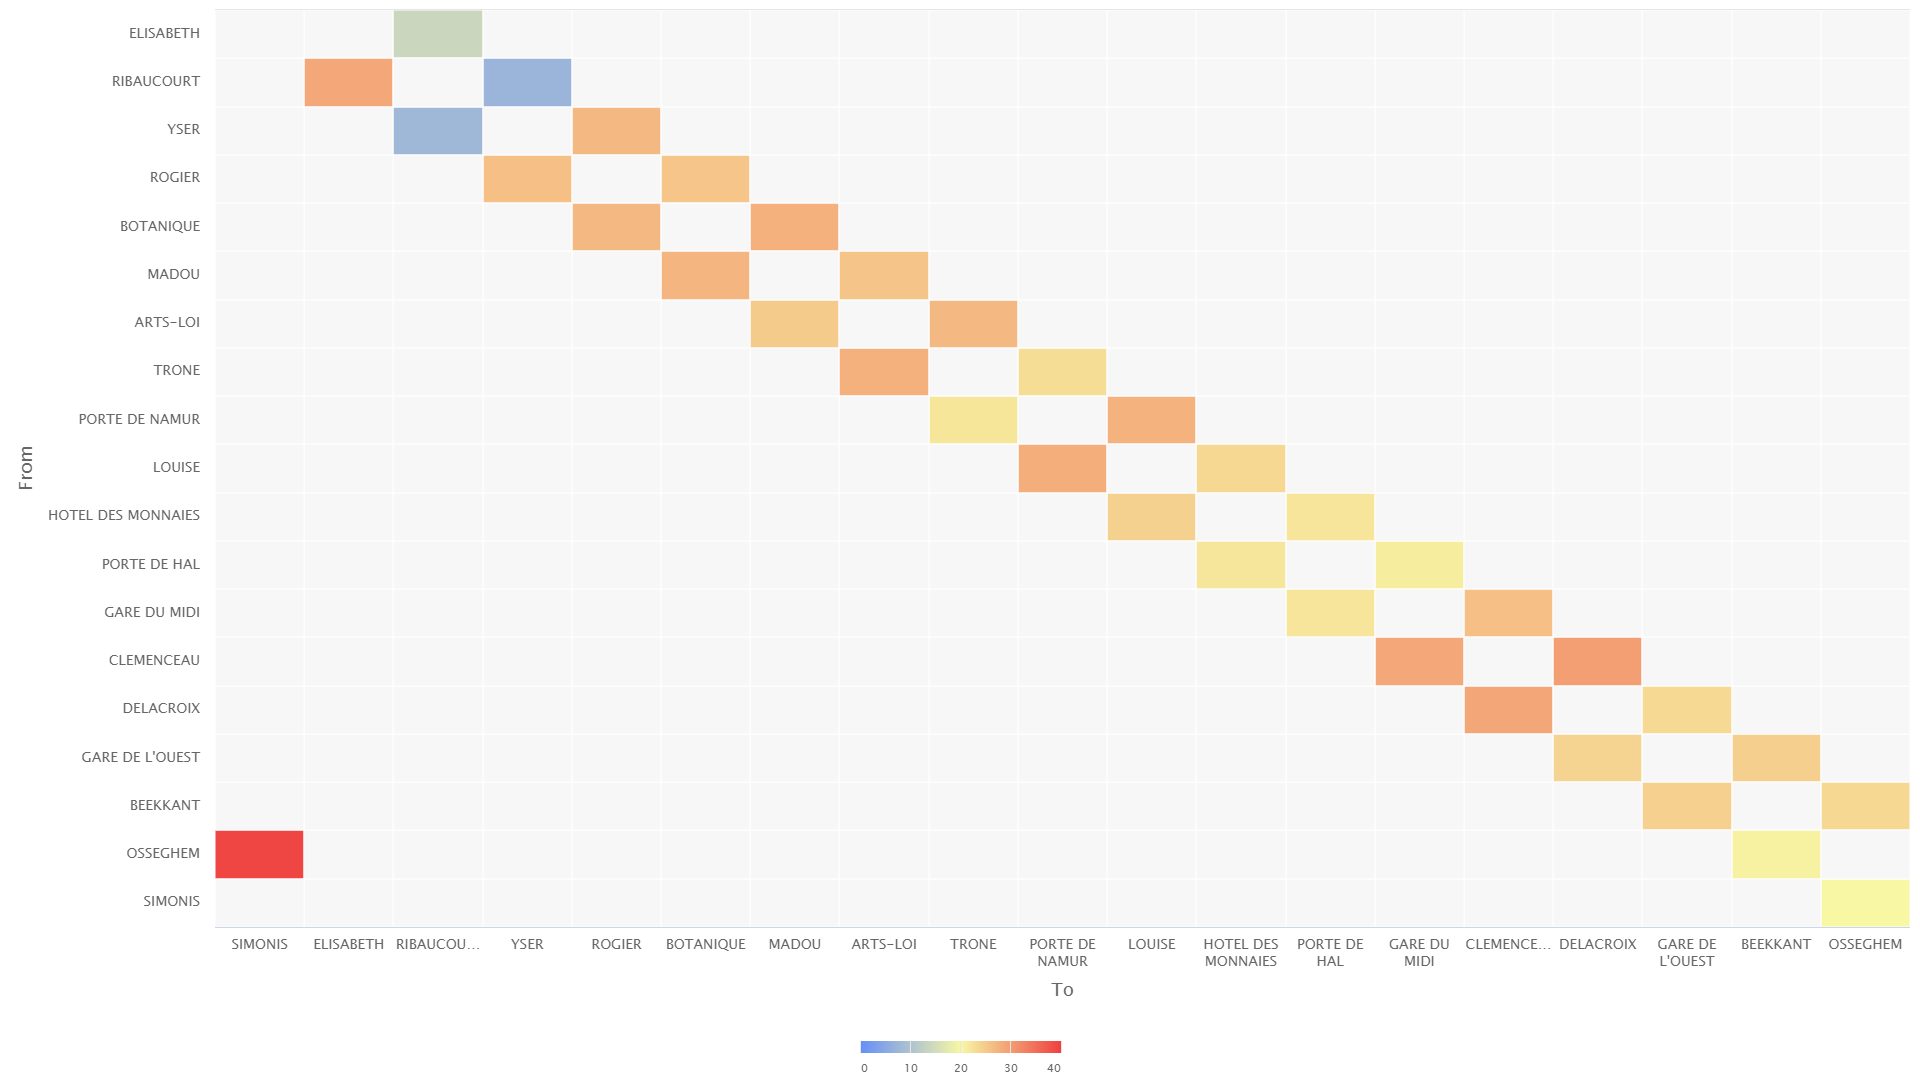
\includegraphics[width=\textwidth]{images/speed_2.png} 
    \caption{Vehicles average speed in km/h over the different segments of line 2}
    \label{fig:speed_2}
\end{figure}

The obtained result indicates that the speed values vary in the range between 0 km/h and 40 km/h with most of values in the interval [20, 30]. The result also shows that traveling by two variants of the same segment does not affect the speed of vehicles since there is not a high difference between them.

 \begin{figure}[H]
    \centering
    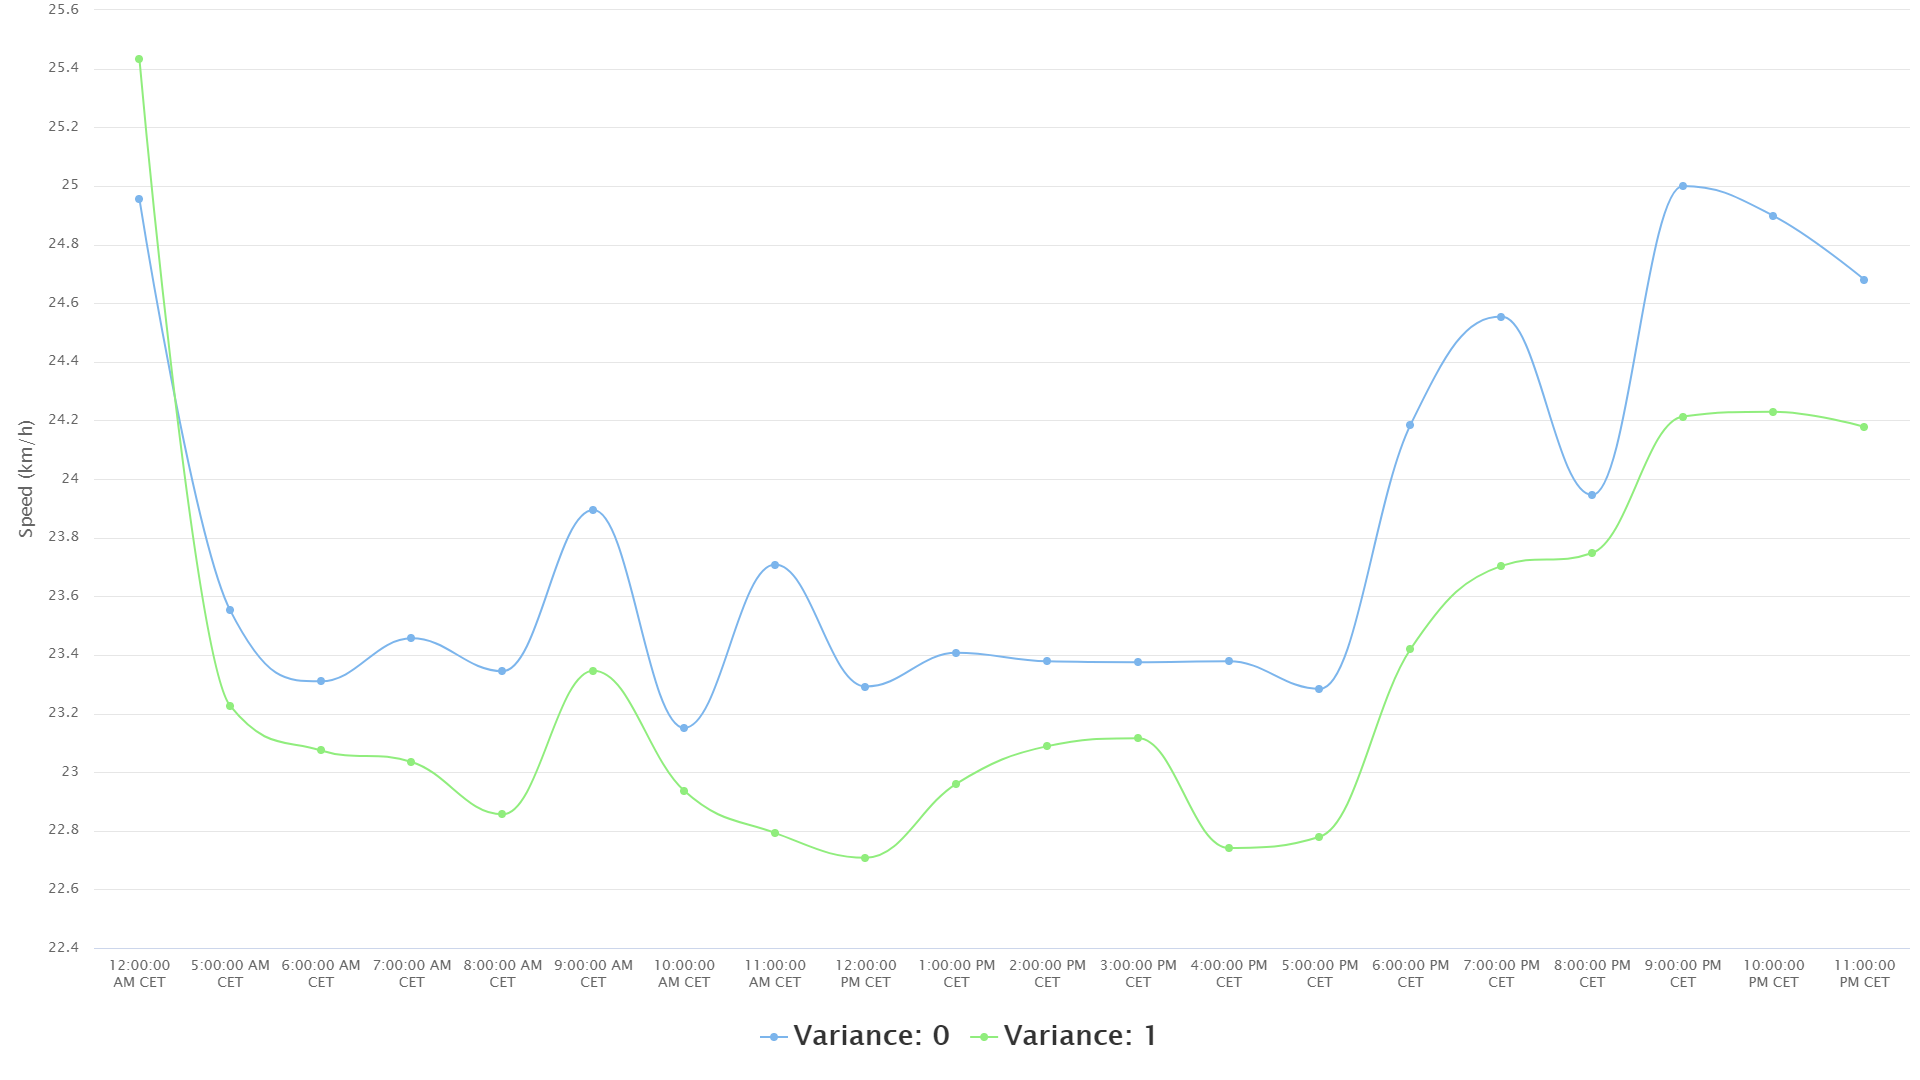
\includegraphics[width=\textwidth]{images/speed_2_hour.png} 
    \caption{Vehicles average speed in km/h over day hours for line 2}
    \label{fig:speed_2_hour}
\end{figure}

In the first sight, a huge peak in the diagram can be observed at 6:00 PM. In fact, from 6:00 PM to 12:00 AM, the average speed of line 2 is higher in both variances compared to other hours. As diagram shows in the range out of 6:00 PM to 12:00 AM, the speed variation is almost between 0 $\frac{km}{h}$ to 1 $\frac{km}{h}$.





\subsubsection{Speed of each transport mode according to weekdays}
The first verification that has been performed, was on speed of each transport mode according to weekdays. To do so, for each day of week, the average of speeds of each transport mode calculated. The result is as follows: 
 \begin{figure}[H]
    \centering
    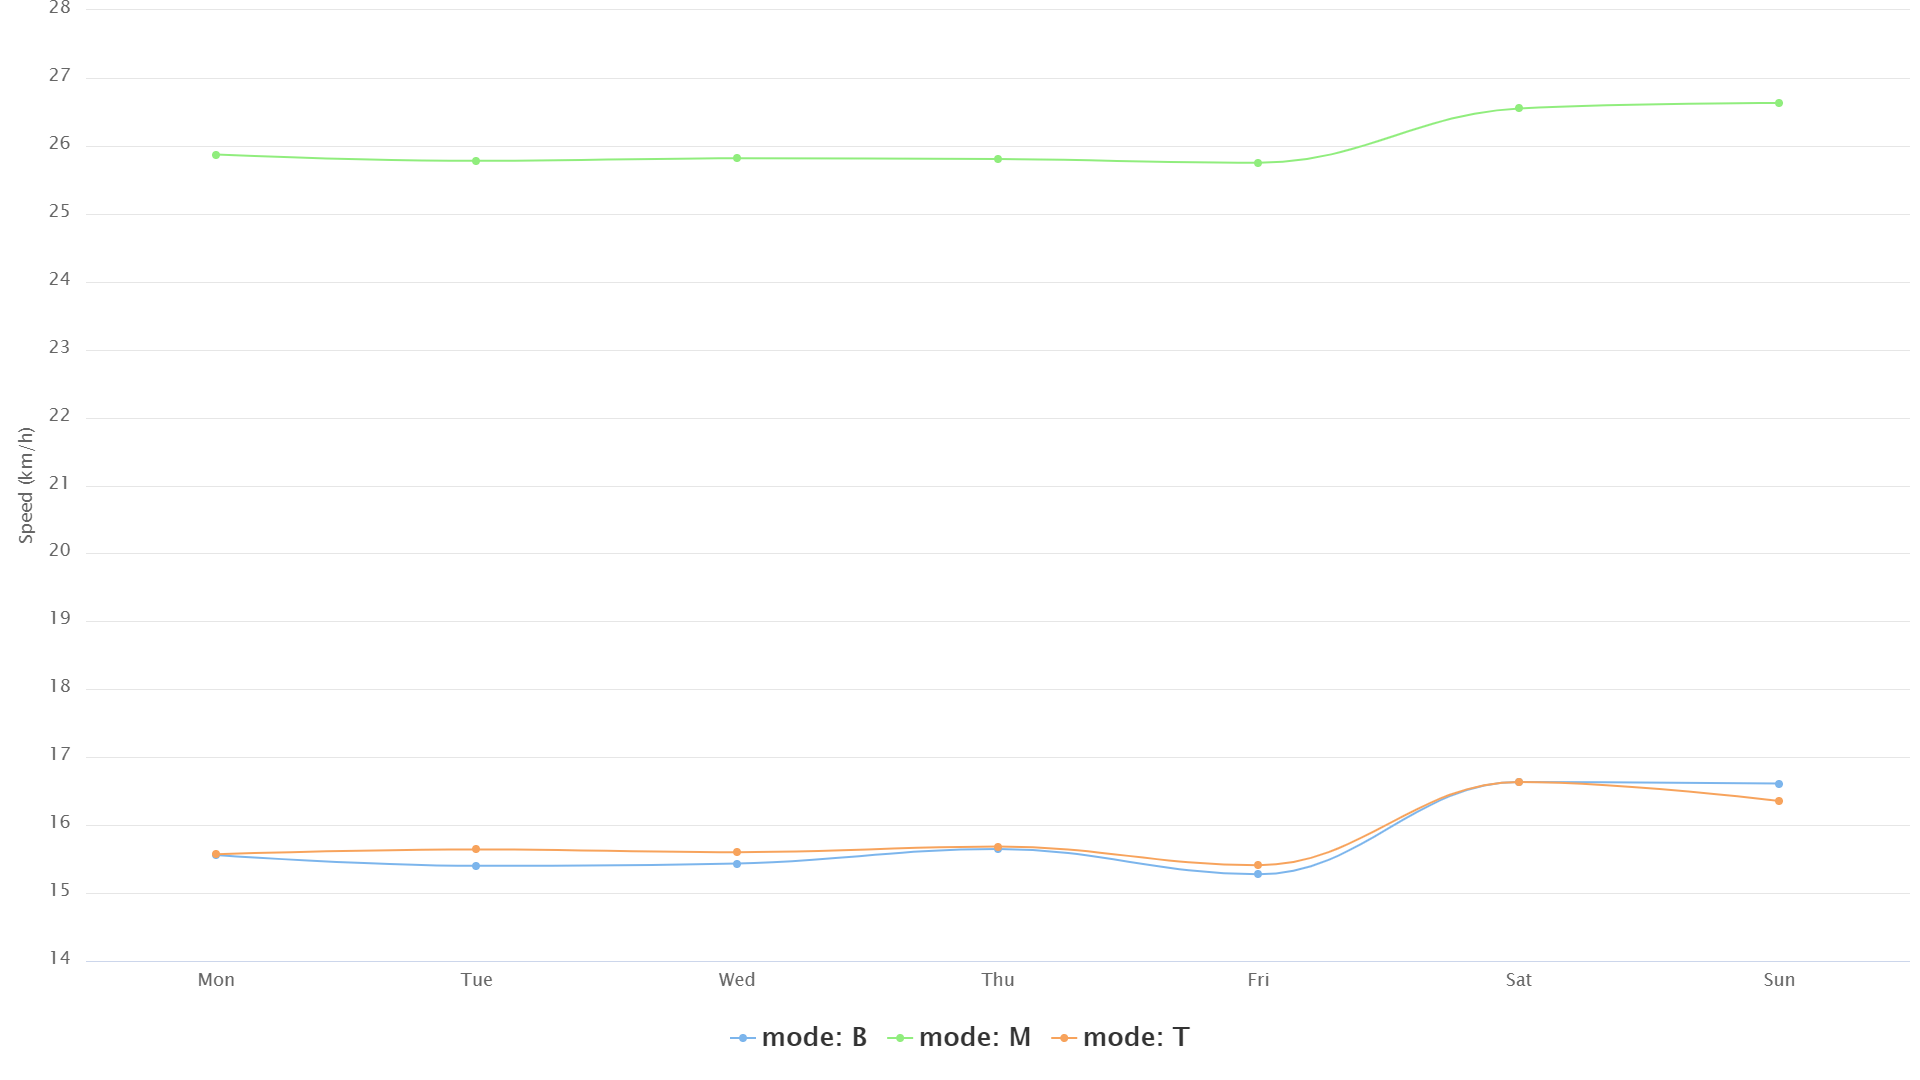
\includegraphics[width=\textwidth]{images/Speed_Day.png} 
    \caption{Transport modes speed according to each day of week}
\end{figure}
An overview of the diagram displays that the metro average speed is at least $10 \frac{km}{h}$ greater than average speed of bus and tram. This can be explained by considering the route that each transport mode, traverse. Metros normally traverse a route underground, so it is away from urban traffic while bus and tram traverse on congested areas of the city.

As the diagram also shows, for all the transport modes, the average speed at weekends (Saturdays and Sundays) is greater than the average speed of other days of week. The reason for that is pretty obvious. In the weekends traffic congestion in the city is lower compared to other days as offices, schools and etc are closed.

Another noteworthy thing about this diagram is that the speed of tram is a little bit more than speed of bus except in the weekends. That can be described by taking into account that the quantity of special routes for trams over the city is greater than the quantity of special routes of buses over the city. But as the weekend traffic congestion decreases, buses can go more rapid compared to trams.

A comparison which can be interesting is, to verify the result that have been calculated by our calculation with the official statistic of STIB \footnote{\url{https://www.stib-mivb.be/irj/go/km/docs/WEBSITE_RES/Attachments/Corporate/Statistiques/2020/STIB_RA2020_Statistiques_EN_web.pdf}}. The average speeds of each transport modes, according to our calculation and STIB statistics are as follows:
\begin{table}[H]
\begin{center}
\begin{tabular}{|c|c|c|c|}
\hline
calculator / transport mode & Metro      & Tram       & Bus        \\ \hline
STIB statistics             & 27.9 km/h  & 16.2 km/h  & 15.5 km/h  \\ \hline
Our calculatuion             & 26.03 km/h & 15.84 km/h & 15.79 km/h \\ \hline
\end{tabular}
\end{center}
\end{table}

The table shows that the calculation that have been made in this project almost corresponds to official statistics of STIB. 


\subsubsection{Speed of each transport mode according to day hours}
The second verification 
performed is on the speed of each transport mode according to hours. To do so, for each hour of a day, the average of speed of each transport mode at that hour is calculated. The result is as follows:
 \begin{figure}[H]
    \centering
    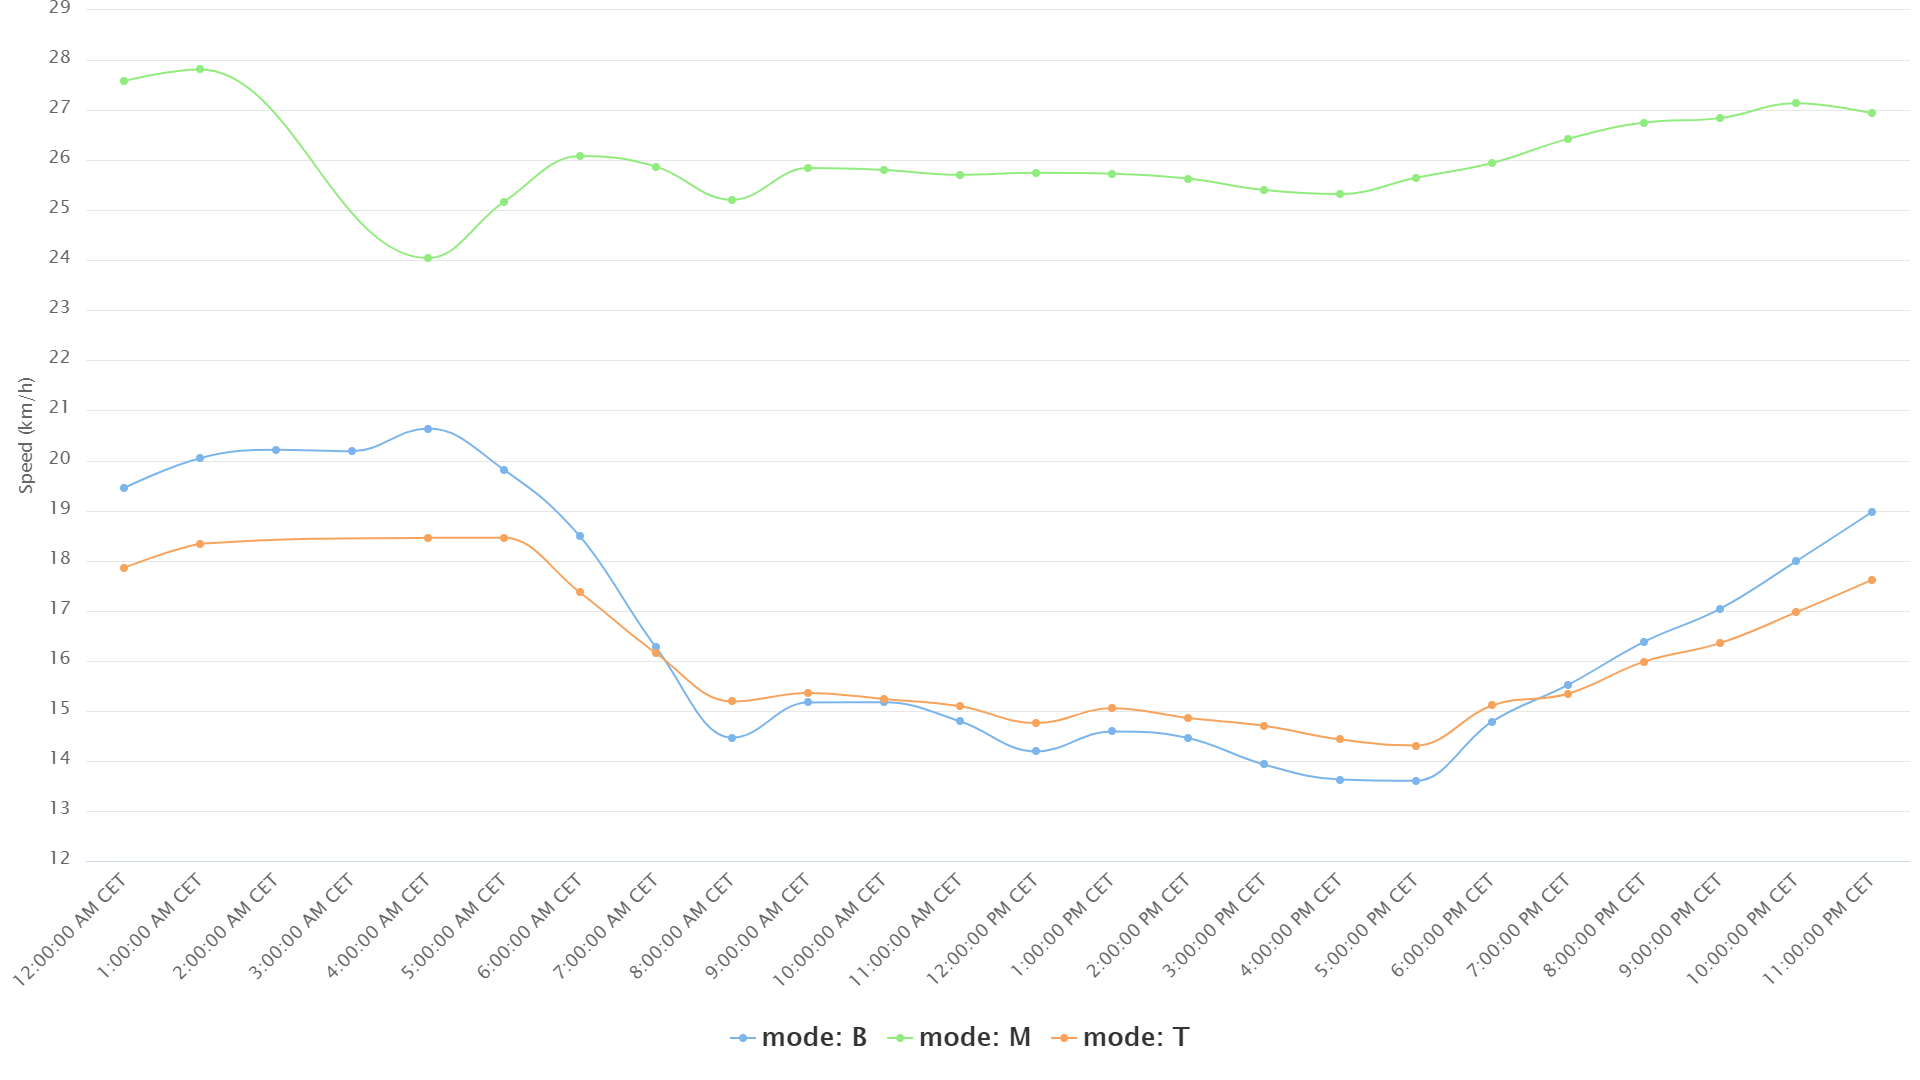
\includegraphics[width=\textwidth]{images/Speed_hour.png} 
    \caption{Transport modes speed according to day hours}
\end{figure}
As the overview shows, metros have less speed variation during the day compared to buses and tramways. In general, the metro is faster than the bus and the tramway. Buses and tramways have almost the same range of variation in the diagrams, but in rush hours, the speed of tramways is higher than the speed of buses. In other hours of the day the bus speed is larger than the tramway speed. The reason of that is the greater quantity of dedicated routes for tramways compared to buses as explained in the previous diagram.

It can be also seen that there exists a speed reduction at 8:00 AM and 5:00 PM in the diagram. These hours are rush hours of a day. As at 8:00 AM people are going to work and students are going to school and as at 5:00 PM offices and schools close, it is normal to have such kind of diagram. Between 8:00 AM and 5:00 PM the speed rises compared to these hours, but it is lower than the speed out of range 8:00 AM to 5:00 PM.


\subsubsection{Metros speed vs. hours}

The below graph (figure \ref{fig:metro}) shows the average speed distribution of metros for each hour of the day. This average speed distribution is calculated for each day of the week.

\begin{figure}[H]
    \centering
    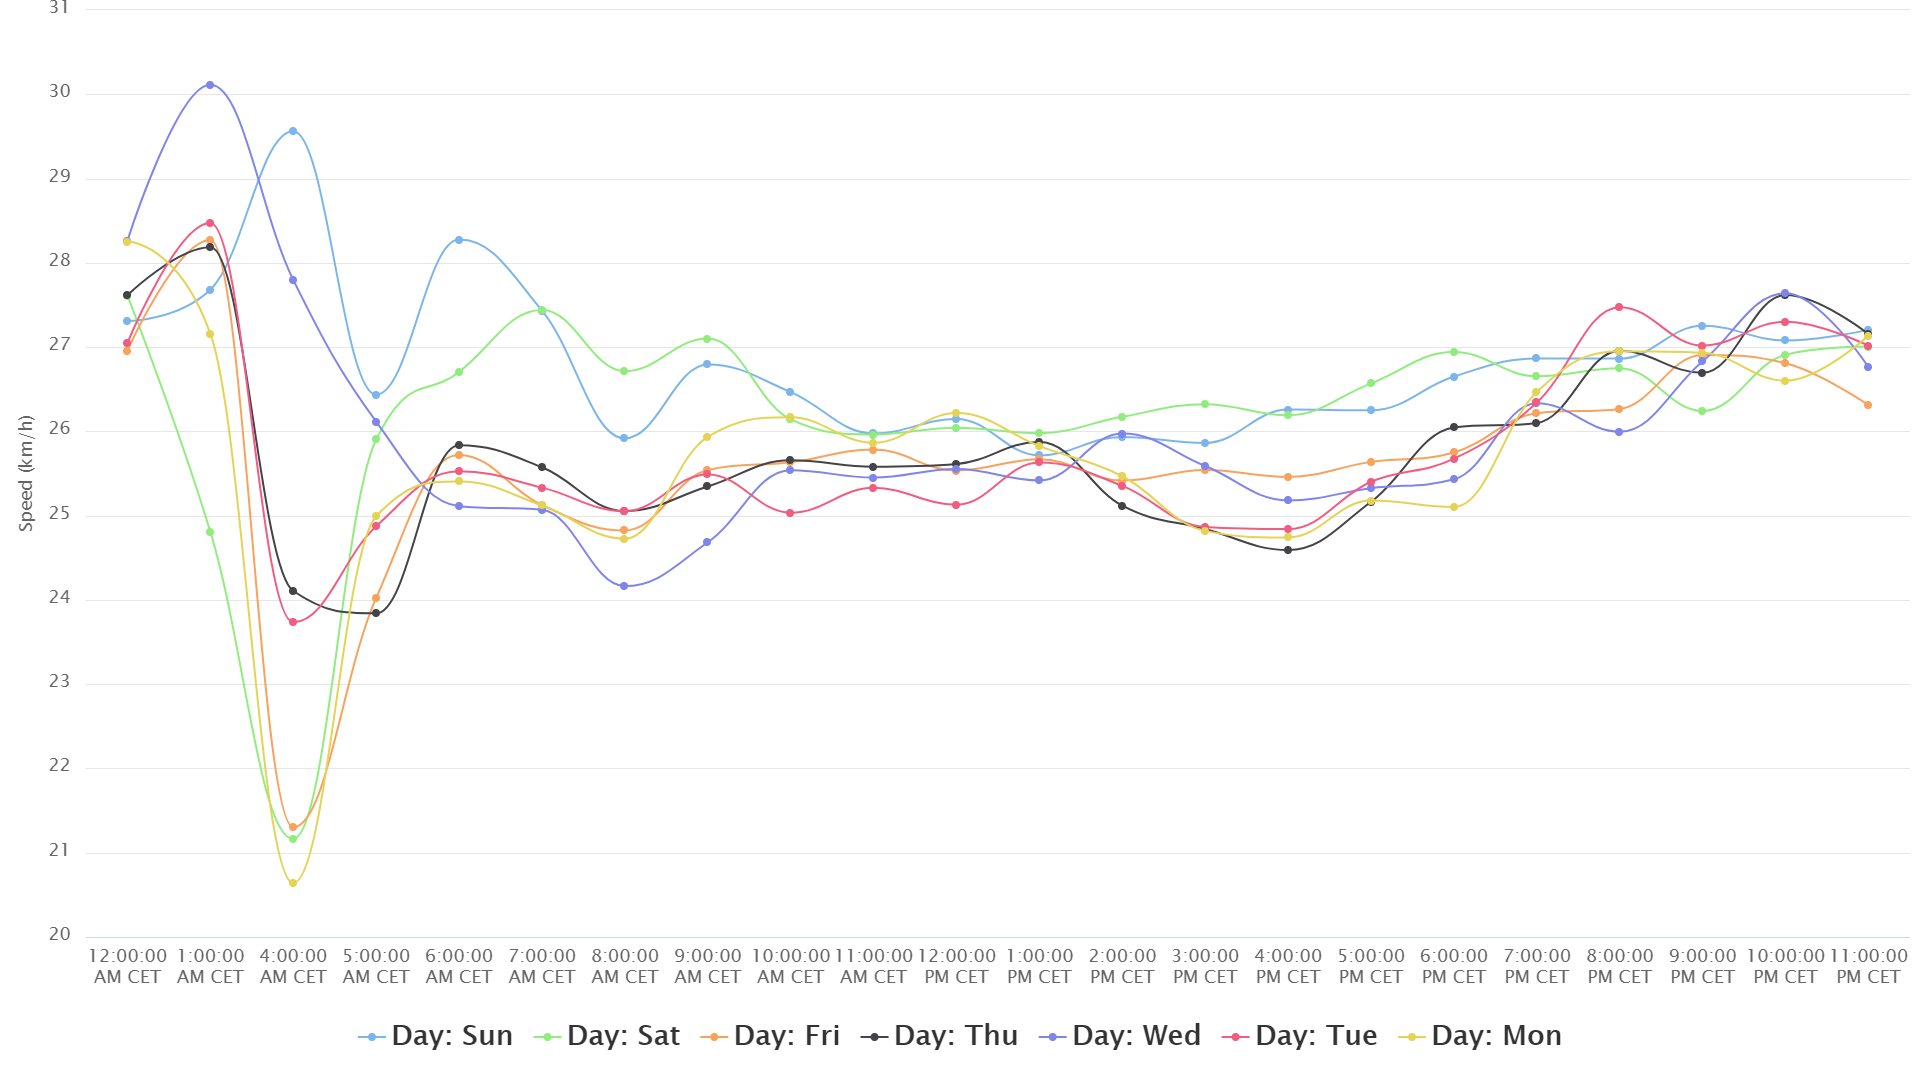
\includegraphics[width=\textwidth]{images/Speed_day_hour_m.png} 
    \caption{metro}
    \label{fig:metro}
\end{figure}

The curves corresponding to Saturdays and Sundays (weekend) show globally higher values of speed than the other days (working days). In addition, each working day show a strong speed reduction at 4:00 AM. This value is to be considered with care because most metro lines do not start before 5:00 AM. This low value comes from very few metros which are starting their daily service and are therefore not representative of the normal operations.

The rest of the day is more interesting with a small reduction of speed around 8:00 AM and around 4:00 PM. The variations are, however, not huge with most average speed values being between 24 km/h and 29 km/h.

\subsubsection{Buses speed vs. hours}

The below graph (figure \ref{fig:bus}) shows the average speed distribution of buses for each hour of the day. This average speed distribution is calculated for each day of the week.

 \begin{figure}[H]
    \centering
    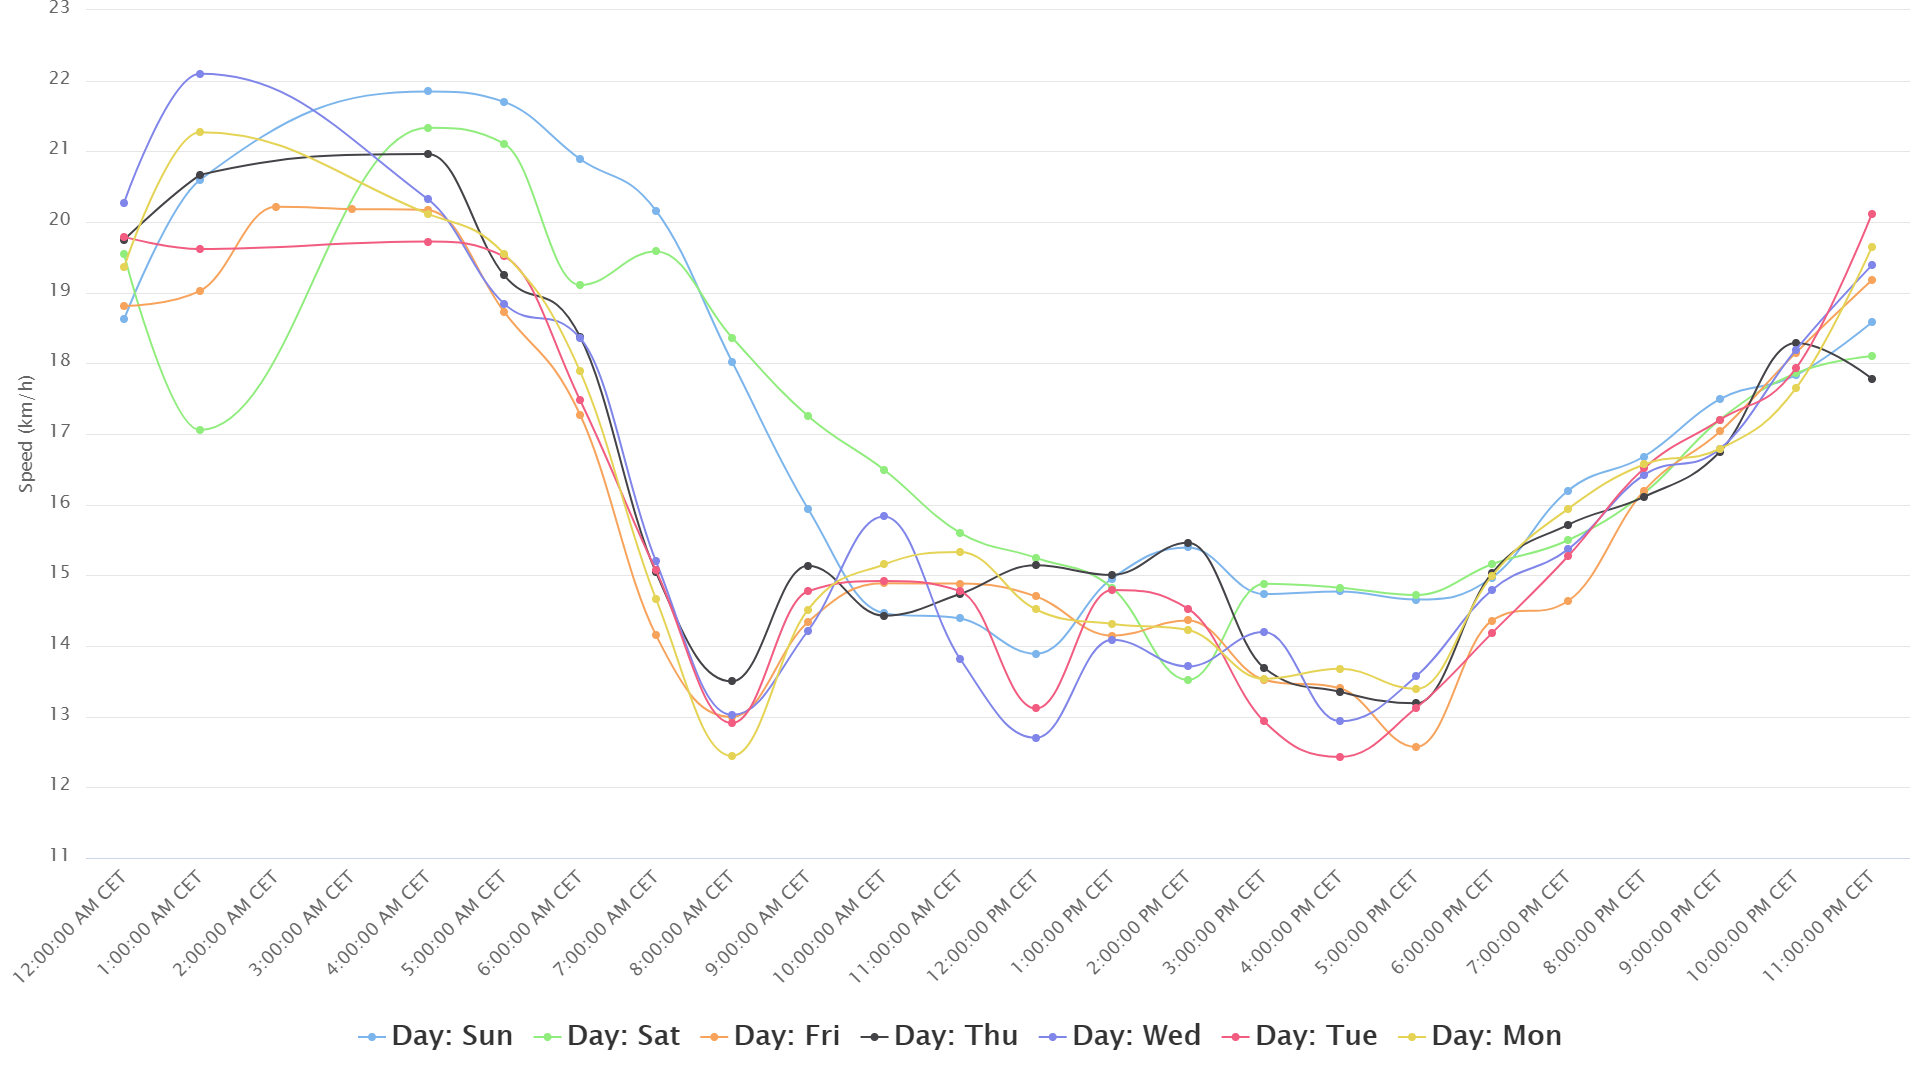
\includegraphics[width=\textwidth]{images/Speed_day_hour_b.png} 
    \caption{bus}
    \label{fig:bus}
\end{figure}

This graph shows higher variations than for metros with values ranging between 22 km/h and 12 km/h. The difference between the weekend and working days is also clearer, especially in the morning. The 8:00 AM reduction of speed during working days is easily identifiable, while it is not present during the weekend. The increase of speed in the evening is very consistent through all days.

\subsubsection{Tramways speed vs. hours}

The below graph (figure \ref{fig:tram}) shows the average speed distribution of tramways for each hour of the day. This average speed distribution is calculated for each day of the week.


 \begin{figure}[H]
    \centering
    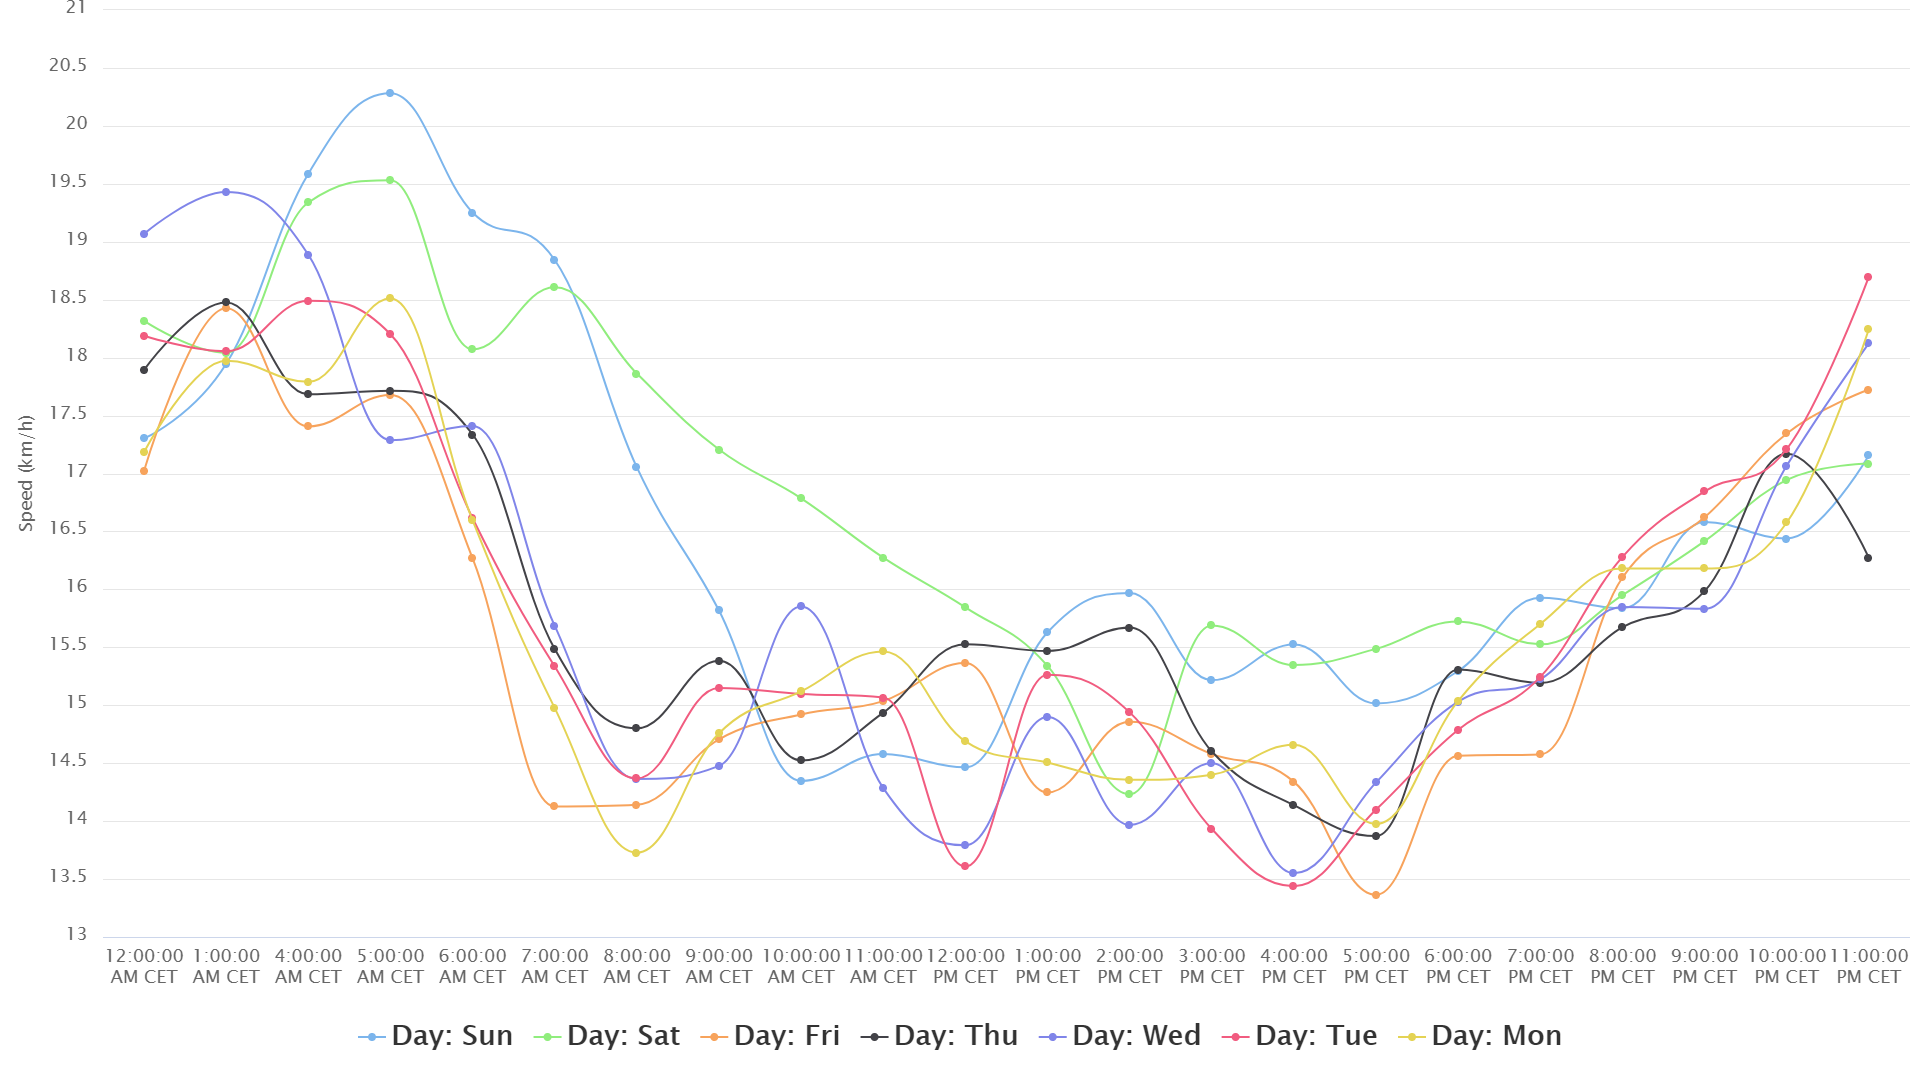
\includegraphics[width=\textwidth]{images/Speed_day_hour_t.png} 
    \caption{tram}
    \label{fig:tram}
\end{figure}

This graph is quite similar to the buses graph with a bit more variation between each working day. The variations during the day are slightly smaller than for buses (between 20 km/h and 13,5 km/h).

\section{Analysis of vehicle delays}

This task consists of analyzing the vehicle delays at the different stops, how it varies across stops, and over time. The following files are required to perform the current task. The duration of the vehicle trips was not fully covered by only one of the GTFS snapshot files, thus both snapshots were used. The explanation of the GTFS files that have been used, comes from the official Google API documentation~\footnote{\url{https://developers.google.com/transit/gtfs/reference\#dataset_files}}.

\begin{center}
\begin{tabular}{|l|l|m{9cm}|} 
 \hline
 Filename & Source & Defines \\ [0.5ex] 
 \hline\hline
vehiclePositionID.csv & Generated from JSON & Vehicles' trips following a variance of the network's lines\\ 
 \hline
routes.txt & gtfs3Sept, gtfs23Sept & Transit routes. A route is a group of trips that are displayed to riders as a single service.  \\
 \hline
trips.txt & gtfs3Sept, gtfs23Sept & Trips for each route. A trip is a sequence of two or more stops that occur during a specific time period.  \\
 \hline
stop\_times.txt & gtfs3Sept, gtfs23Sept & Times that a vehicle arrives at and departs from stops for each trip.  \\
 \hline
calendar.txt & gtfs3Sept, gtfs23Sept & Service dates specified using a weekly schedule with start and end dates. \\
 \hline
calendar\_dates.txt  & gtfs3Sept, gtfs23Sept & Exceptions for the services defined in the calendar.txt. \\
 \hline
\end{tabular}
\end{center}

\subsection{Data processing}

The source data does not contain trip information, therefore, to determine the delay of each vehicle, it is necessary to match each vehicle trip to one of the possible trips which exist at the same time period. 

First of all, it is important to generate a new \texttt{calendar.txt} file to take into account the exceptions defined in \texttt{calendar\_dates.txt}. This file contains the services which should be modified, their modification date and the type of modification. Value 1 means that the service has been added for the specified date while value 2 means that the service has been deleted for the specified date.

For instance, by using the \texttt{calendar\_dates.txt} and \texttt{calendar.txt} files, the obtained result is represented by the new \texttt{calendar.txt}. This exception handling process can be seen below:

\begin{lstlisting}[caption={calendar\_dates.txt},captionpos=b]
service_id,date,exception_type
238162502,20210920,1
238074051,20210927,2
238074051,20210928,2
238074051,20210929,2
238074051,20210930,2
238074051,20211004,2
238074051,20211005,2
238074051,20211006,2
238074051,20211007,2
238074051,20211011,2
238074051,20211012,2
238074051,20211013,2
238074051,20211014,2
\end{lstlisting}

\begin{tabular}{p{8.6cm}|p{8.6cm}}

\hspace{3.6cm} Before & \hspace{3.6cm} After \\
\vspace{0.8cm}
\begin{lstlisting}[caption={calendar.txt},captionpos=b]
service_id,monday,tuesday,wednesday,thursday ,friday,saturday,sunday,start_date,end_date
238162502,0,0,0,0,0,1,0,20210918,20210919
238074051,1,1,1,1,1,0,0,20210924,20211015
\end{lstlisting}

&

\begin{lstlisting}[caption={new calendar.txt},captionpos=b]
service_id,monday,tuesday,wednesday,thursday ,friday,saturday,sunday,start_date,end_date
238162502,0,0,0,0,0,1,0,20210918,20210919
238162502,0,0,0,0,0,1,0,20210920,20210920
238074051,1,1,1,1,1,0,0,20210924,20210926
238074051,1,1,1,1,1,0,0,20211001,20211003
238074051,1,1,1,1,1,0,0,20211015,20211015
\end{lstlisting}

\end{tabular}

Once the first step is completed, the next step is to select only the useful information fields in each file. The result is as follows:

\begin{itemize}
    \item \texttt{vehiclePositionID.csv} : All fields (i.e., Time, LineID, Variance, DirectionID, pointID and distanceFromPoint).
    \item \texttt{calendar.txt} : All fields (i.e., service\_id, ``Days of week", start\_date and end\_date).
    \item \texttt{routes.txt} : route\_id and route\_short\_name (i.e., LineID).
    \item \texttt{trips.txt} : route\_id, trip\_id, service\_id and direction\_id (i.e., Variance).
    \item \texttt{stop\_times.txt} : trip\_id, stop\_id and arrival\_time.
\end{itemize}

As the selected fields show, the theoretical travel time and the real travel time cannot be linked directly. It is therefore important to join the files together to create the missing link. Thus, these files have been used to generate these links and to simplify understanding. The fields are renamed as follows:
\begin{itemize}
    \item Vehicles = \{\texttt{vehiclePositionID.csv}\} : Time, VehicleID, LineID, Variance, DirectionID, pointID and distanceFromPoint.
    \item Calendar = \{\texttt{calendar.txt, routes.txt, trips.txt}\} : service\_id, ``Days of week", start\_date, end\_date, LineID, and Variance.
    \item Stop Times = \{\texttt{stop\_times.txt, routes.txt, trips.txt}\} : trip\_id, stop\_id and arrival\_time, service\_id, LineID, and Variance.
\end{itemize}

\begin{figure}[H]
    \centering
    \begin{minipage}{0.5\textwidth}
        \centering
        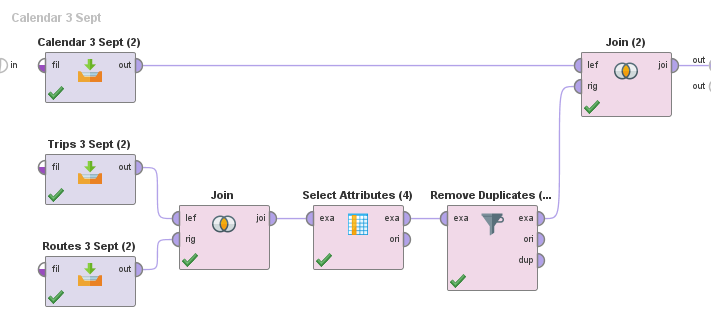
\includegraphics[width=0.9\textwidth]{images/Superset Calendar.png}
        \caption{Calendar}
    \end{minipage}\hfill
    \begin{minipage}{0.5\textwidth}
        \centering
        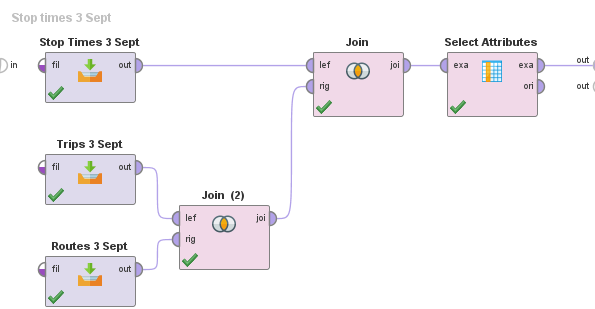
\includegraphics[width=0.9\textwidth]{images/Stops Times Superset.png} 
        \caption{Stop Times}
    \end{minipage}
\end{figure}

Now that these links are created, things get more interesting. As the result shows, each vehicle trip can be matched to one of the possible trips. For this purpose, a filtering is performed on the vehicles as shown below:

\begin{figure}[H]
    \centering
    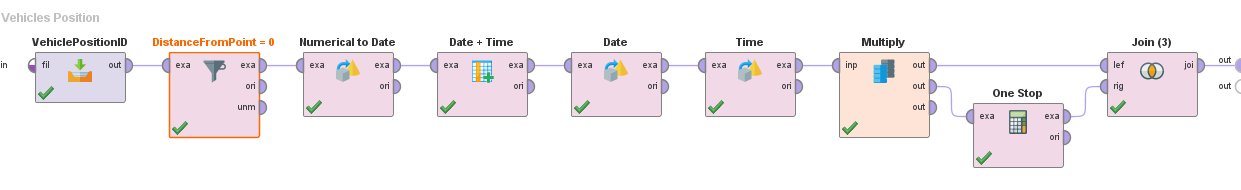
\includegraphics[width=\textwidth]{images/Vehicles Filter.png} 
    \caption{Vehicles filtering}
\end{figure}


\begin{enumerate}
    \item Filter vehicle trips to obtain only the entries for which the vehicle position is exactly the same as the position of a stop (i.e., distanceFromPoint = 0).
    \item Keep only one entry for each different stop (i.e., the one with the earliest time) because it is this entry which represents the arrival time.
\end{enumerate}

 After filtering the vehicles, the following phase consists in extracting from the calendar each possible service in the same period as the one in which the trips were made, then assigning it to each vehicle belonging to the same line variance as that of the service. Among all the possibilities that have been obtained, filtering was applied to retain only the valid services (i.e., the service which is available on the same day as the given trip).
 
 \begin{figure}[H]
    \centering
    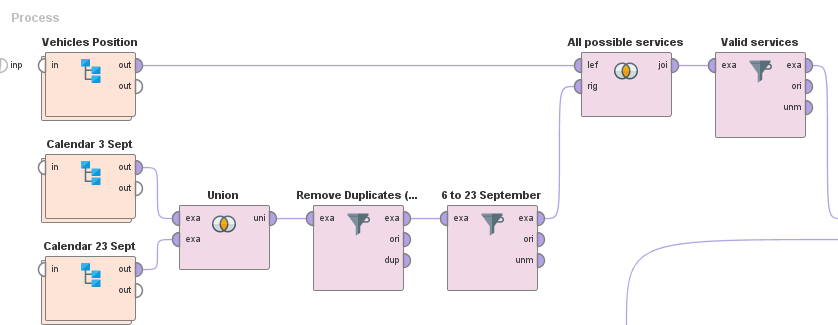
\includegraphics[width=\textwidth]{images/First join.png} 
    \caption{Linking vehicles to services}
\end{figure}

At this stage of the process, the information obtained is all the possible services that a trip can have. This service information is used to connect a real trip to all the theoretical trips which belong to the stops schedule.

 \begin{figure}[H]
    \centering
    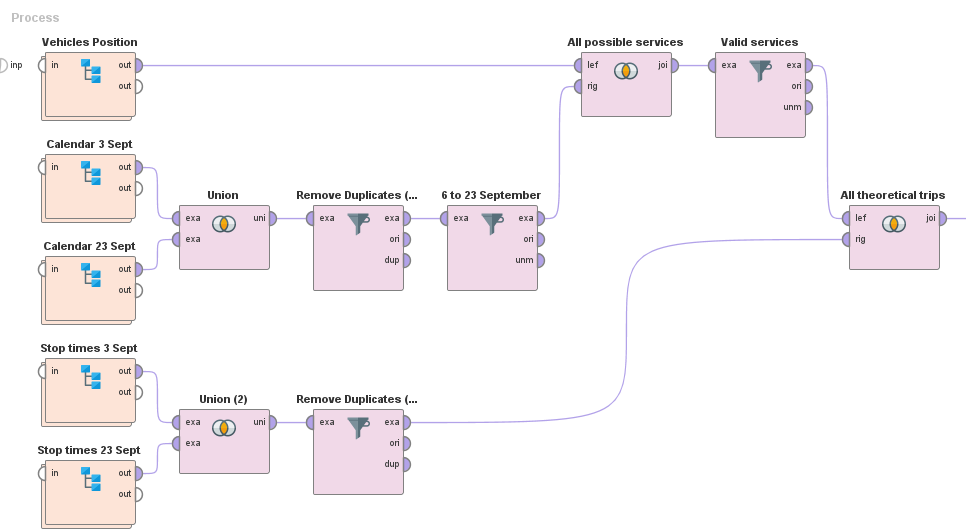
\includegraphics[width=\textwidth]{images/Second join.png} 
    \caption{Linking vehicles to theoretical trips}
\end{figure}

Now that each real route is linked to one or more theoretical trips, the most accurate one must be picked. The chosen approach is to pick only those that cover all the stops of the trip. Note that some vehicle trips are temporary or exceptional (i.e., they do not appear on the schedule). Therefore, they are not taken into account. Afterwards, the real trip is compared to all the remaining ones by computing the overall delay with respect to each trip and choosing the one with the lowest delay value.

 \begin{figure}[H]
    \centering
    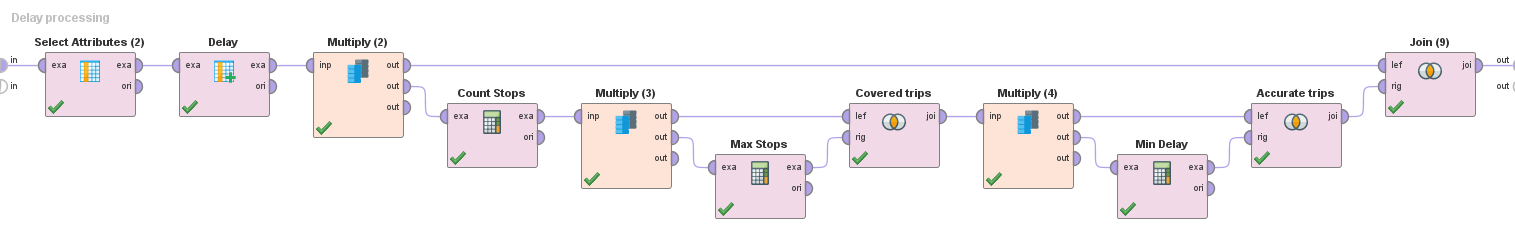
\includegraphics[width=\textwidth]{images/Delay.png} 
    \caption{Delay processing}
\end{figure}

Note that the method of computing the delay is as follows: the difference between the theoretical time and the real time is calculated in absolute value (i.e., arriving before the scheduled time is also considered as a delay).

All the steps explained are grouped in this complete process below:

 \begin{figure}[H]
    \centering
    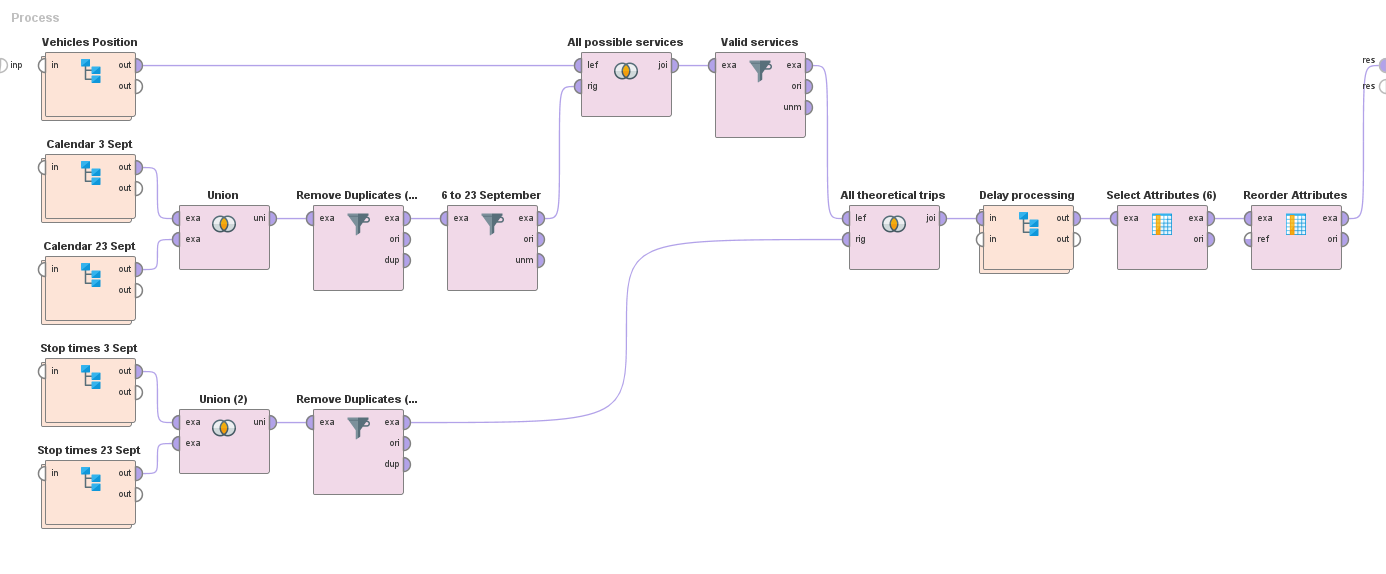
\includegraphics[width=\textwidth]{images/Model.png} 
    \caption{Complete process}
\end{figure}

\subsection{Results}
For this section, the analysis has been performed on a specific line as the analysis of all lines together was not possible due to limited amount of available memory. The diagrams below, show the result that has been obtained for line 2 which is a metro line with 19 stops in both of its variances.


 \begin{figure}[H]
    \centering
    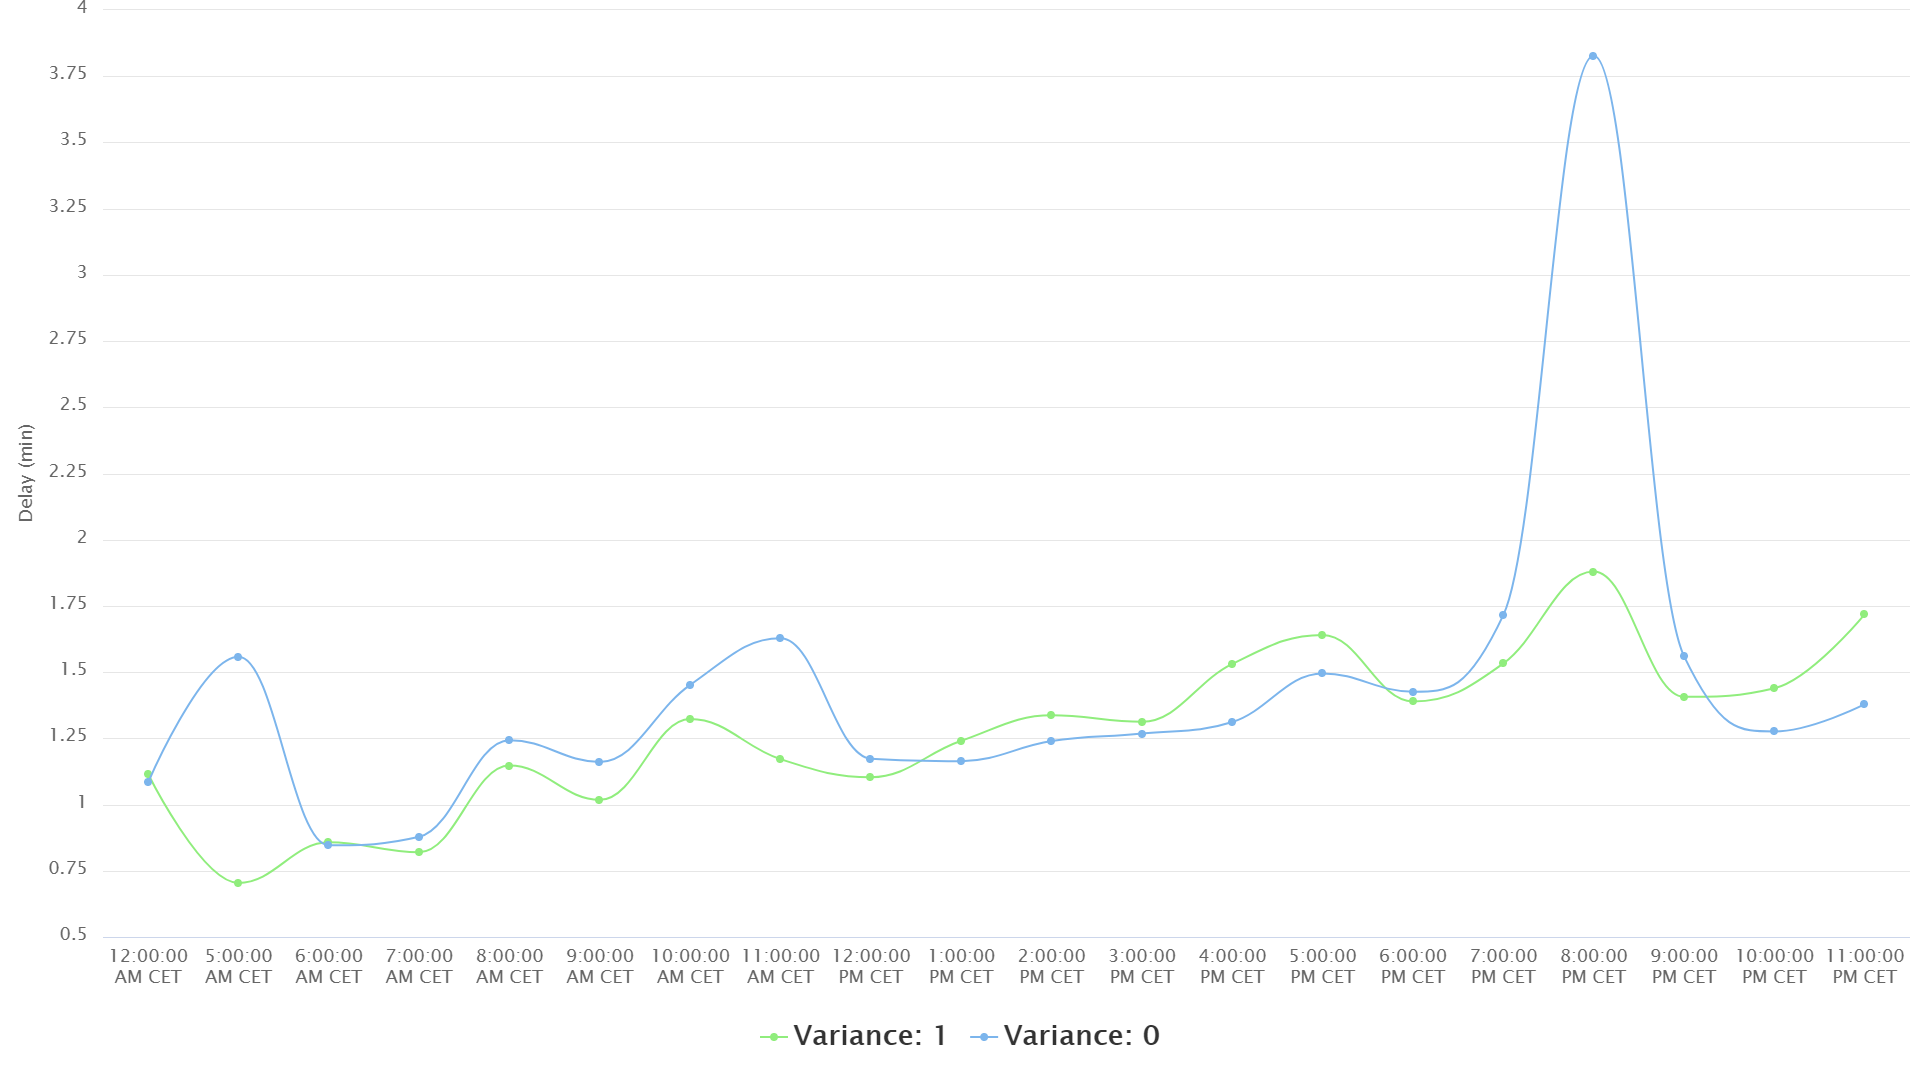
\includegraphics[width=\textwidth]{images/delay_2.png} 
    \caption{Total delay of line 2 per hour}
    \label{fig:delay_2}
\end{figure}
As figure \ref{fig:delay_2} shows, there exists a peak at 8:00 PM in diagrams in both variances. This shows that at 8:00 PM this metro line is more crowded compared to other hours. Something which is interesting is that at this hour, delay of the first variance is almost 2 minutes more than delay of second variance, in average. So, it can be concluded that first variance of line 2 is more crowded at the evening, compared to its second variance. 

General overview on the diagram shows that in average there exists a delay between 1 to 2 minutes, in each hour in average. This delay is tolerable considering that other lines and transport modes also have almost the same range of delay as line 2.

 \begin{figure}[H]
    \centering
    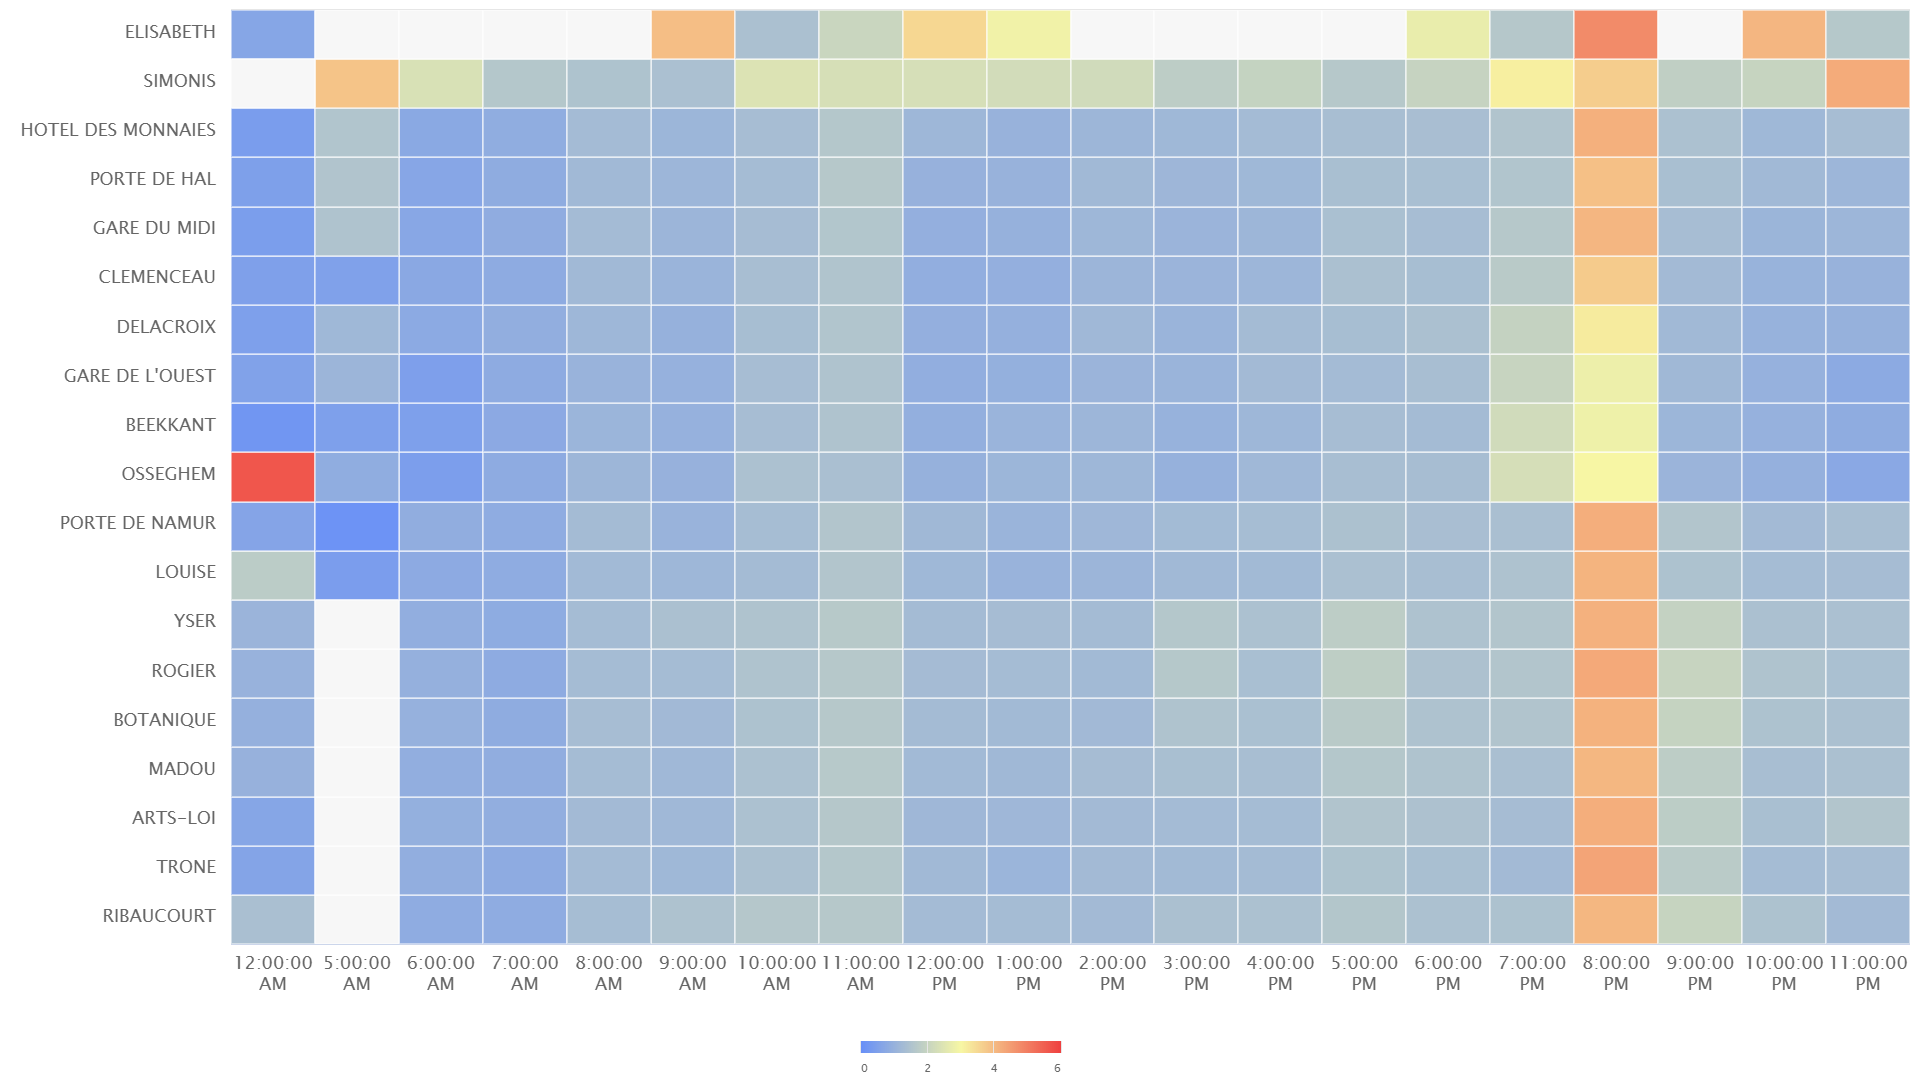
\includegraphics[width=\textwidth]{images/delay_2_stop_hour_0.png} 
    \caption{Line 2 variance 0 stops delay per hour}%{variance 0}
\end{figure}
 \begin{figure}[H]
    \centering
    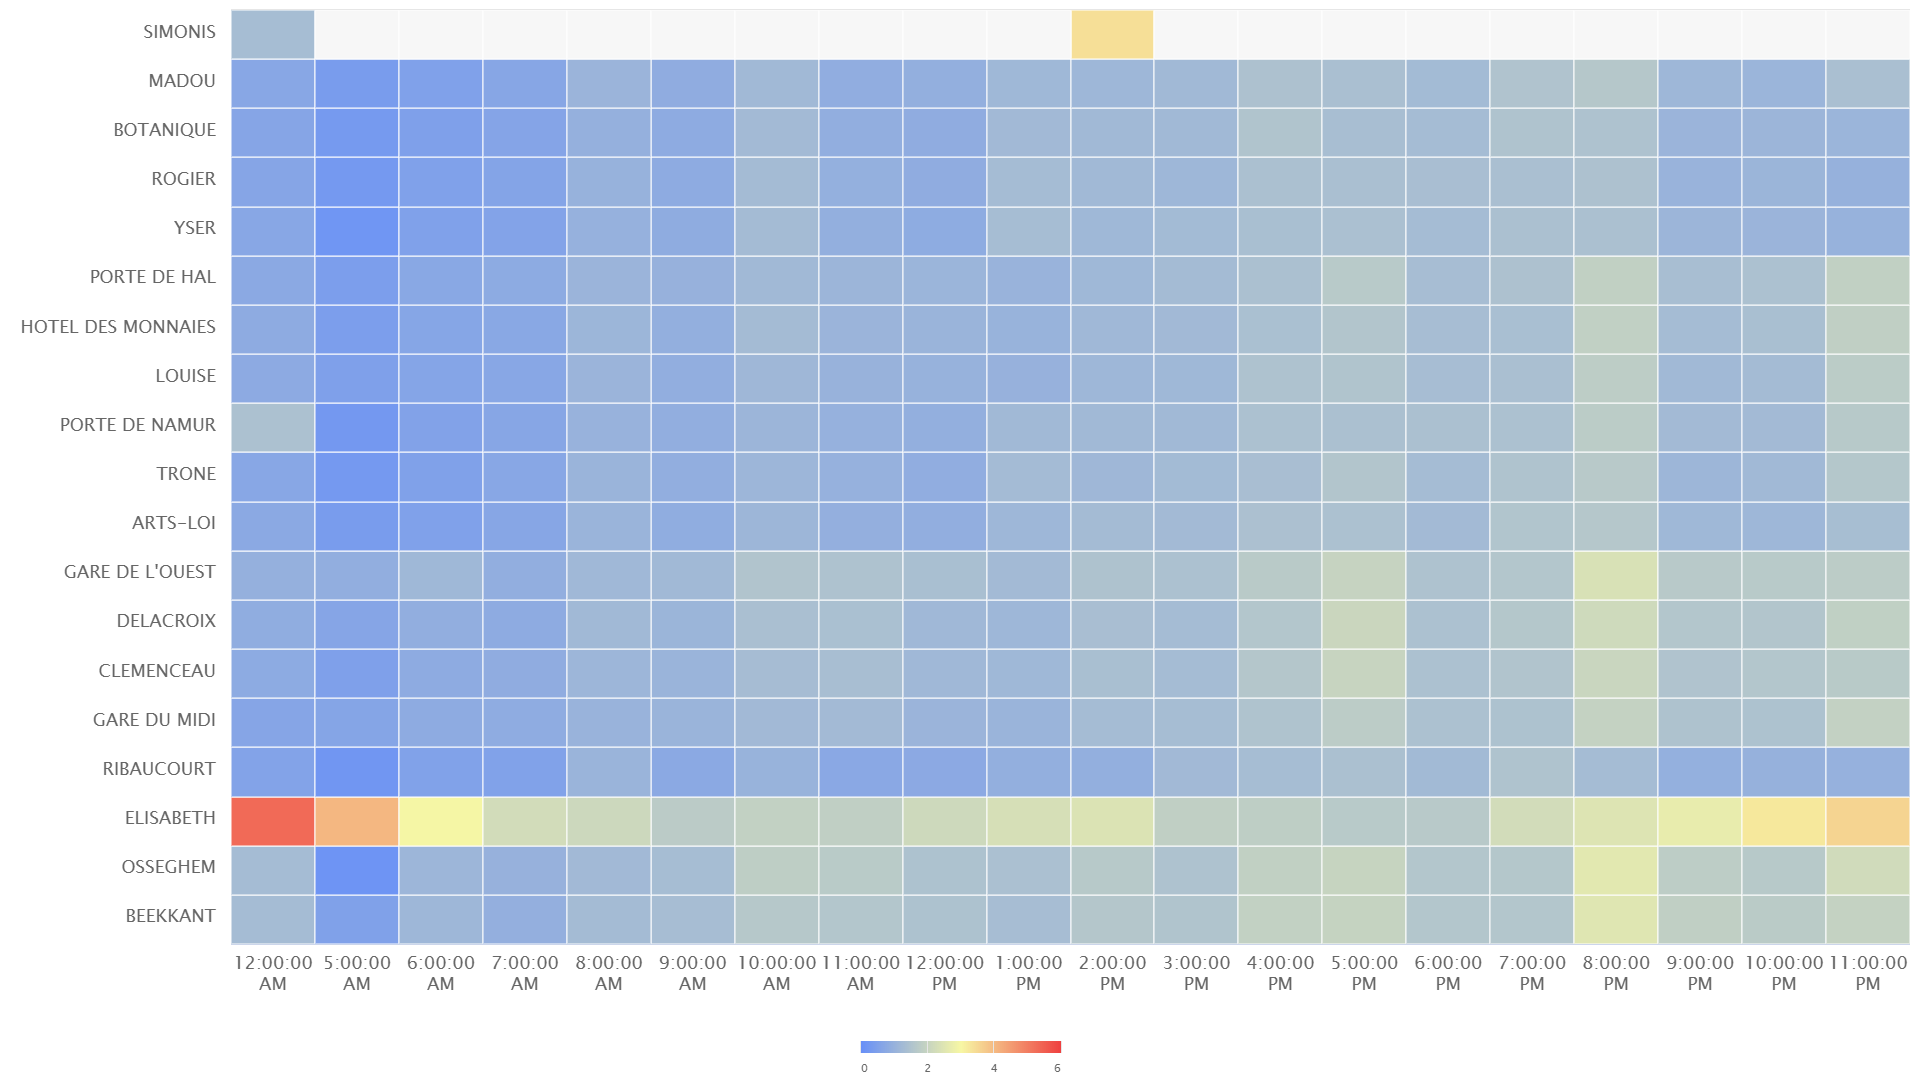
\includegraphics[width=\textwidth]{images/delay_2_stop_hour_1.png} 
    \caption{Line 2 variance 1 stops delay per hour}
\end{figure}

The two diagrams are mostly blue which indicates that, the range of delay is almost between 0 and 2 minutes for each stop. It can be mentioned that in both diagram the average delay in the first stop (Simonis for variance 0 and Elisabeth for variance 1) is higher compared to other stops of the line. Maybe by decreasing this initial delay at first stops, STIB reaches a more exact time schedule with lower minutes of delay compared to the actual schedule.

 \begin{figure}[H]
    \centering
    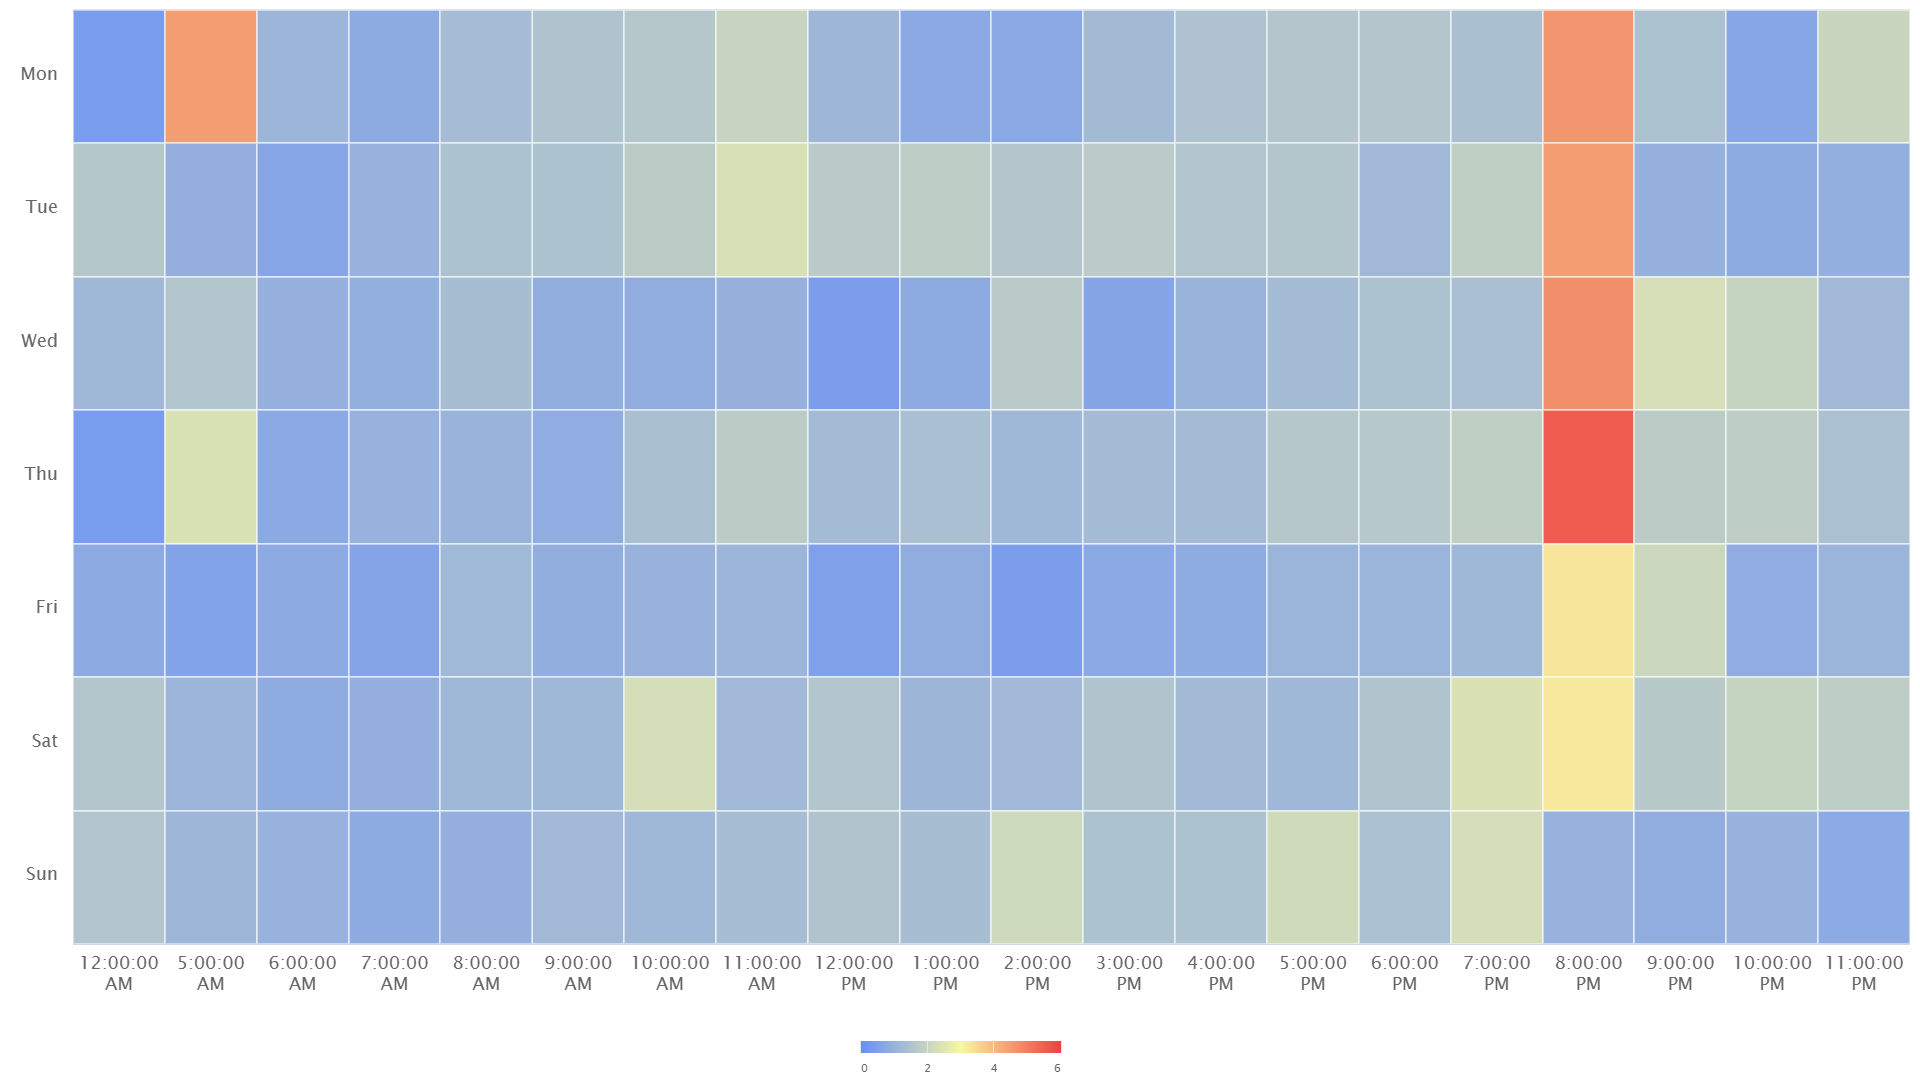
\includegraphics[width=\textwidth]{images/delay_2_day_hour_0.png} 
    \caption{Line 2 variance 0 according to weekdays and hours}
\end{figure}

 \begin{figure}[H]
    \centering
    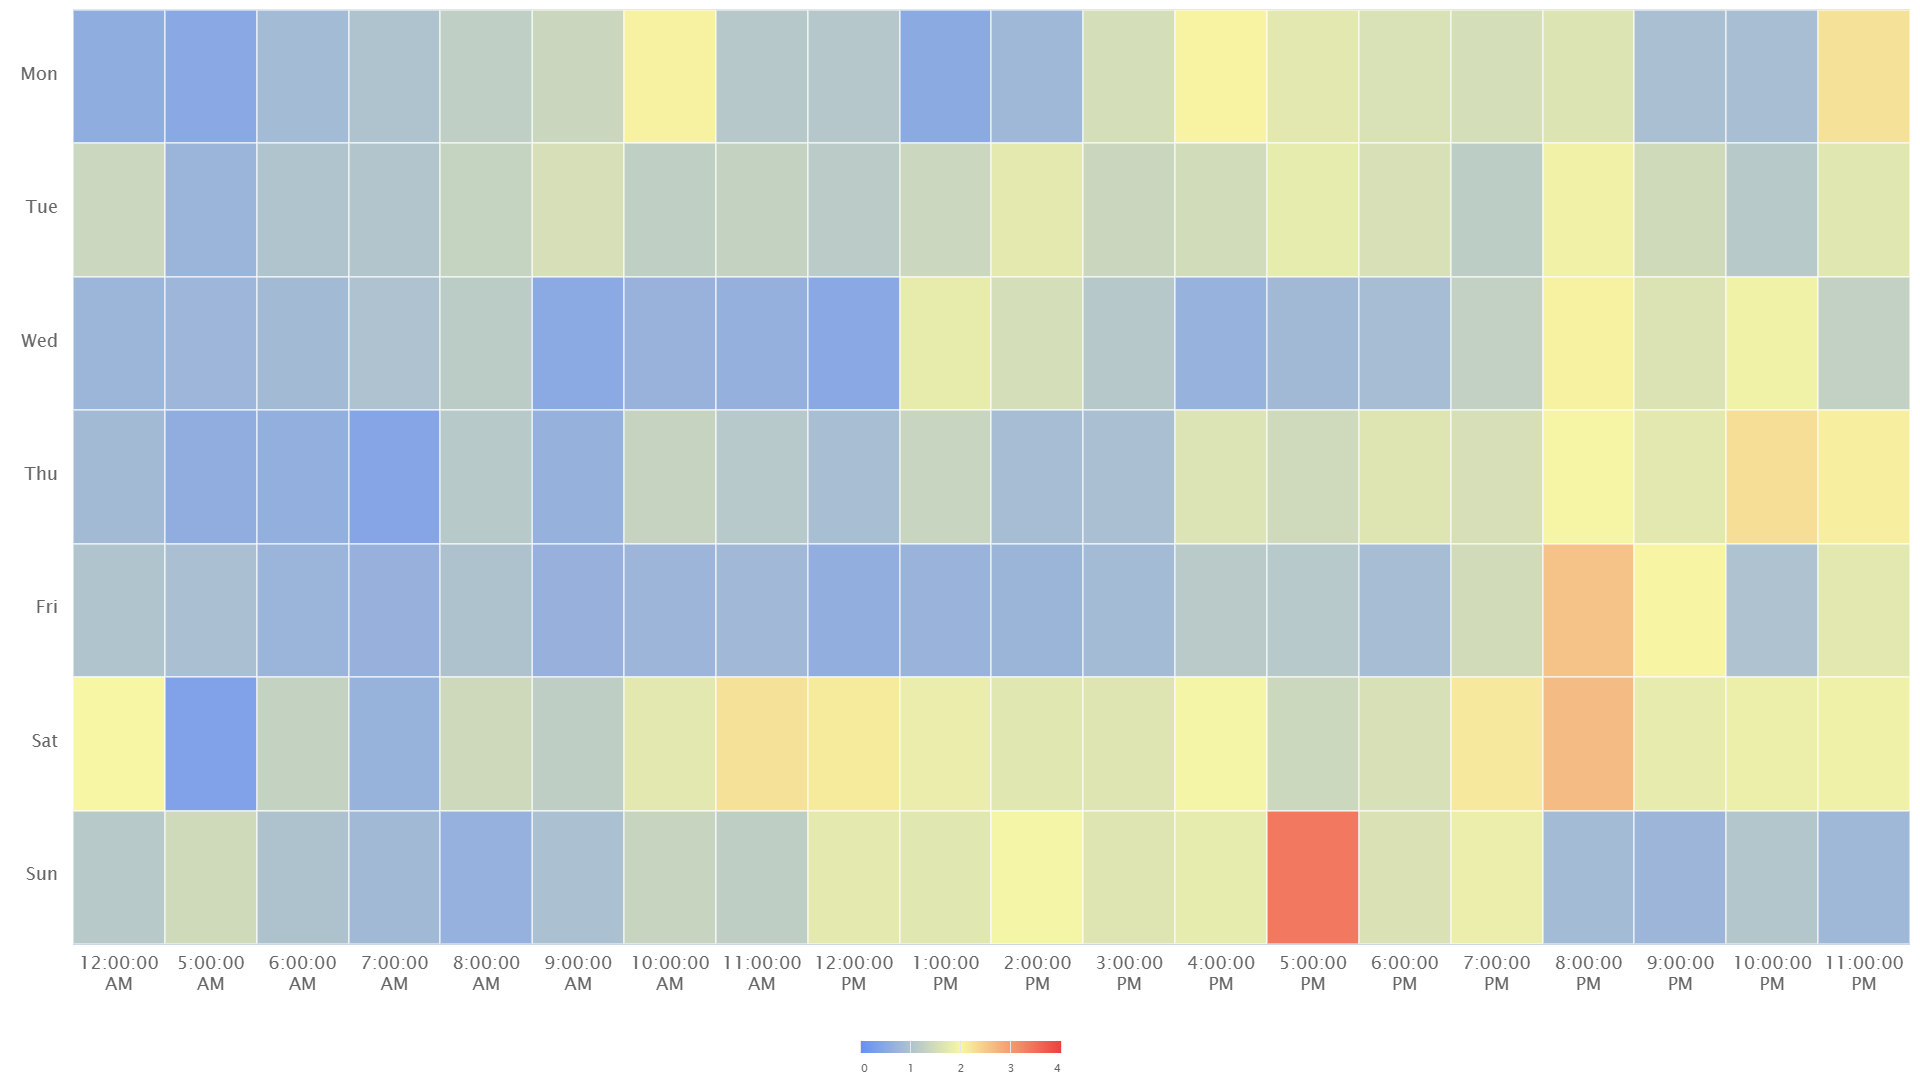
\includegraphics[width=\textwidth]{images/delay_2_day_hour_1.png} 
    \caption{Line 2 variance 1 according to weekdays and hours}
\end{figure}

An overview of the diagrams shows that in the afternoon, there exist more delay compared to the morning. It can also be observed that the variance one has greater delay in average compared to the variance 0 as it has more yellow cases.

As diagrams shows, in average, the total delay on Saturdays and Sundays in both variances is greater than any other days. The reason of that can be explained by considering that during the weekend, the metro line is crowded a greater portion of the day compared to the other days.
 
\section{Arrival time forecasting}

In this part of the project, it is requested to do arrival time forecasting at a given stop in the route of a vehicle, given this vehicle start time. It is also requested to test the accuracy of the forecasting by randomly splitting the dataset in disjoint training and testing subsets.

\subsection{Data processing}

This question is solved using RapidMiner, based on the \texttt{vehiclePositionID.csv} file. The elaborated RapidMiner process follows the below mentioned steps:

\begin{enumerate}

\item Request the considered line number, the variant (direction), the start stop and the end stop as input.

\item Remove ``duplicates", i.e. the vehicle IDs which appear several times in a row at distance 0 from the considered stop. We only keep the first time at the stop (the arrival time).

\item Join the Start stop data to the end stop data.

\item Calculate the time difference between start stop and end stop for each vehicle.

\item Keep only the arrival time and the time difference.

\item Generate new attributes:
    \begin{itemize}
     \item \texttt{Hour} : Integer containing departure time hour.
     \item \texttt{Day} : Integer containing departure time day of the month.
     \item \texttt{Time\_in\_minute}s : Time difference in minutes.
    \end{itemize}

\item Calculate the averages of the time differences in minutes for every hour in the data to obtain a computable time series.

\item Fill in the missing values with zeroes (for night time or any other time frame without any measurements).

\item Generate an ID in order to be able to make some operations on the time series.

\end{enumerate}

\subsection{Results}

\subsubsection{Data exploration}
To learn a bit more about the generated time series, the following operations are performed:
\begin{enumerate}
    \item Fast Fourier Transformation
    \item STL decomposition
    \item Autocorrelation
    \item Partial autocorrelation

\end{enumerate}

In the following paragraphs, the example of Metro line 2, variant 1, from stop \textit{Hôtel des Monnaies} to stop \textit{Clémenceau}, is chosen for illustration.

\textbf{Stationarity}  : it is clear that, just like the speed time series, the time difference time series are clearly stationary (see figure \ref{fig:timeseries}, below). There is therefore no need to convert it to a new time series that would be stationary.

As a reminder, the data covers the whole range of days provided in the input \texttt{JSON} files and it is ranging from the 3\textsuperscript{rd} September to the 23\textsuperscript{rd} September 2021. Each point (id) is an hour. The zero values correspond to hours without any vehicle measurements between start stop and end stop.

 \begin{figure}[H]
    \centering
    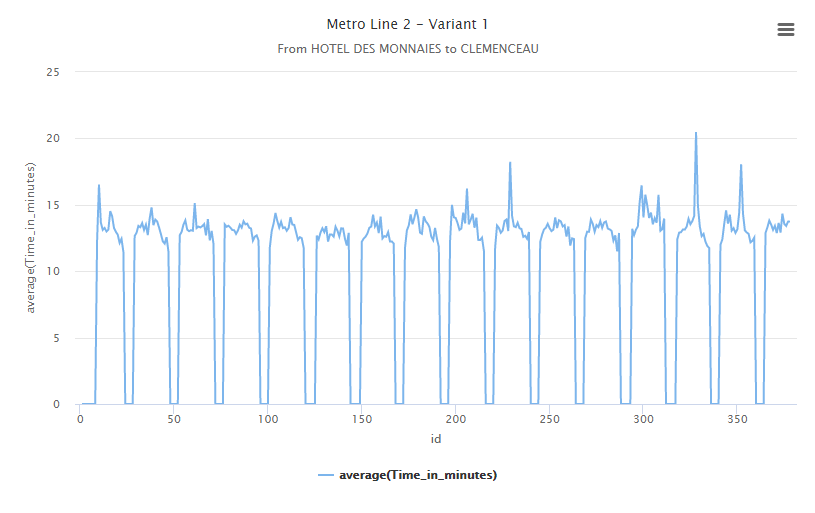
\includegraphics[width=\textwidth]{images/Fig1.png} 
    \caption{Time series}
    \label{fig:timeseries}
\end{figure}

\textbf{FAST FOURIER TRANSFORMATION (FFT)} : The Fast Fourier transformation changes the data from a time-based data to a frequency-based data in order to identify the underlying patterns. In particular, it can help identify the seasonality in time series. As shown in figure \ref{fig:fft}, below, the first peak in seasonality has a frequency of 0,04308 hour\textsuperscript{-1}, which corresponds to a period of 23,2 hours, i.e. quite close to an intuitively significant seasonality : 24 hours. Interestingly enough, there are 2 other easily identifiable seasonal peaks at 0,08225 hour\textsuperscript{-1} and 0,12533 hour\textsuperscript{-1}. These 2 peaks correspond to 12,2 hours (close to half a day) and 7,98 hours (close to a third of a day).

 \begin{figure}[H]
    \centering
    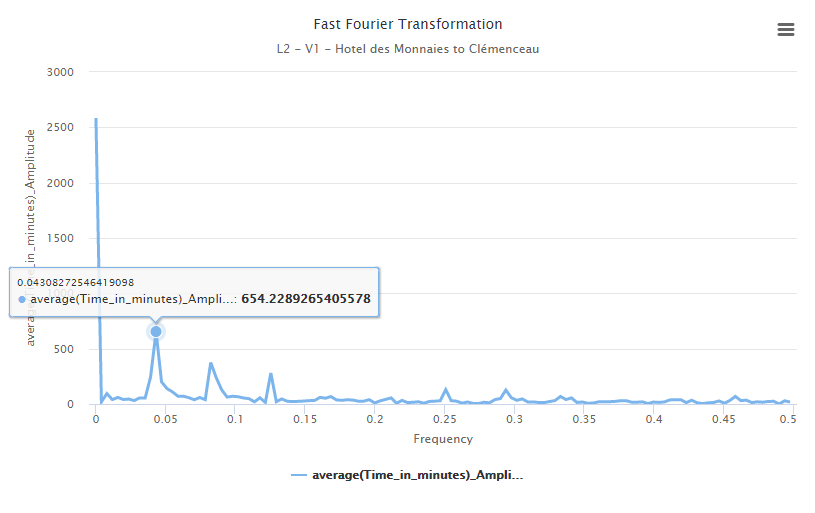
\includegraphics[width=\textwidth]{images/Fig2.png} 
    \caption{Fast Fourier transformation}
    \label{fig:fft}
\end{figure}


\textbf{STL DECOMPOSITION} : STL decomposition (Seasonal and Trend decomposition using Loess) helps identify the seasonal component, the trend, the remainder and potentially the cycles. The selected seasonality is an output of the FFT.

Based on the observation of the FFT, we can therefore use seasonality = 24 in the STL decomposition.

 \begin{figure}[H]
    \centering
    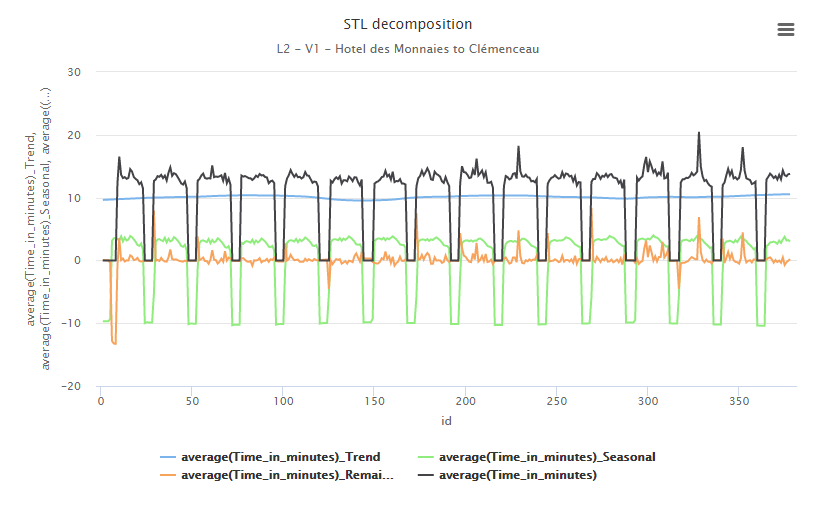
\includegraphics[width=\textwidth]{images/Fig3.png} 
    \caption{STL Decomposition}
    \label{fig:stl}
\end{figure}

Based on figure \ref{fig:stl}, it can be noted that the trend of the time differences (blue curve) is a rather flat curve with little variation over the days. It is visible that the seasonal component (green curve) explains most of the variance. The remainder (black curve), however, remains quite large especially at the early stages of the measurements.

\textbf{AUTOCORRELATION} : Autocorrelation (as a function of time difference L) is the ratio between covariance of a term and the term at t + L and the variance of this term. It corresponds to the correlation between adjacent timestamps in the time series. Is used to define q in the ARIMA model.
 
 \begin{figure}[H]
    \centering
    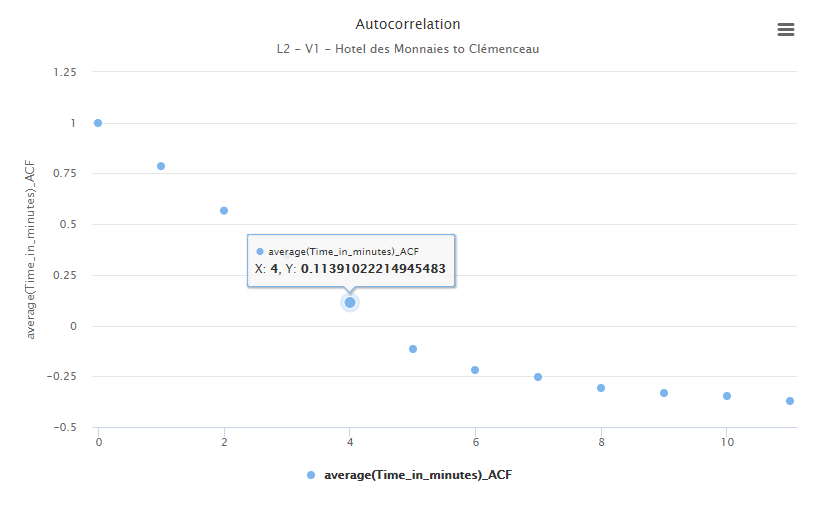
\includegraphics[width=\textwidth]{images/Fig4.png} 
    \caption{Autocorrelation}
    \label{fig:autocor}
\end{figure}
 
 As shown in figure \ref{fig:autocor}, above, the 4\textsuperscript{th} neighbor in the time series still explains more than 11\% of the variance. We will therefore set q = 4 for this specific time series.
 
 
 
\textbf{PARTIAL AUTOCORRELATION} : Partial autocorrelation is the amount of correlation between the term at time t and the term a time t+L which is not explained by the correlation between the term at time t and the ones located between t and t+L. Is used to define p in the ARIMA model.

 \begin{figure}[H]
    \centering
    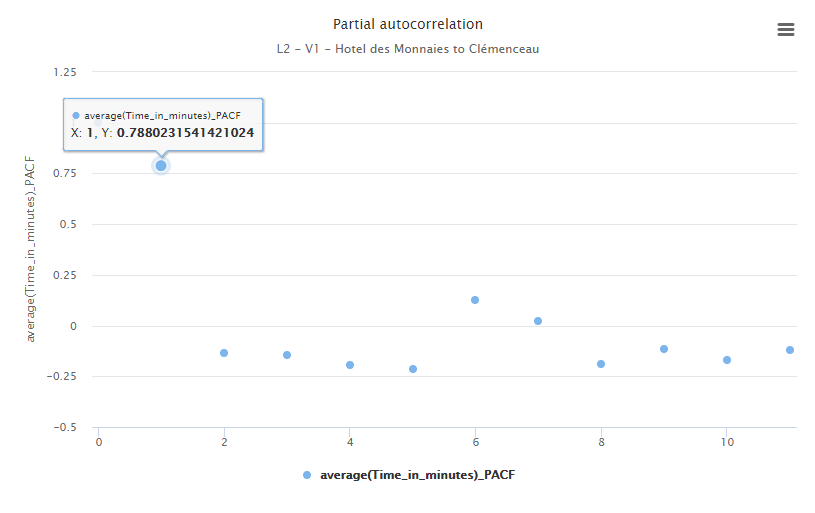
\includegraphics[width=\textwidth]{images/Fig5.png} 
    \caption{Partial autocorrelation}
    \label{fig:part-autocor}
\end{figure}

 As shown in figure \ref{fig:part-autocor}, above, the 1\textsuperscript{st} neighbor in the time series has a direct impact on the value of the considered value, but the 2\textsuperscript{nd} neighbor already has no impact other than the one explained by the correlation between the one considered and the 1\textsuperscript{st} neighbor. We will therefore set p = 1 for this specific time series.
 
It should be noted that these p and q parameters should be checked for every time difference series computed.

\subsubsection{ARIMA forecast}
In order to perform ARIMA forecasting, and as requested in question 3 of this project, it was required to "test the accuracy of [our] forecasting by randomly splitting the given dataset in disjoint training and testing subsets". Forecast validation was therefore performed in RapidMiner. A window size of 120 hours (training set) and a step size of 1 hour were selected. The horizon size (test set) was set to 5 hours.

These input parameters, as well as the p = 1, d = 0 (stationary time series) and q = 4, give a Root Mean Squared Error of 3,898 minutes, an Absolute Error of 3,354 minutes and a relative error of 17,72\%. Let us be clear, these results are not as accurate as one would have liked.

These accuracy figures are given for a main criterion being AIC (Akaike information criterion). Choosing BIC (Bayesian information criterion) or AICC (AIC with correction for small sample sizes) does not drastically modify the accuracy of the model.

The forecast validation graph shown in figure \ref{fig:valid}, below, illustrates the differences between the model and the actual data.

 \begin{figure}[H]
    \centering
    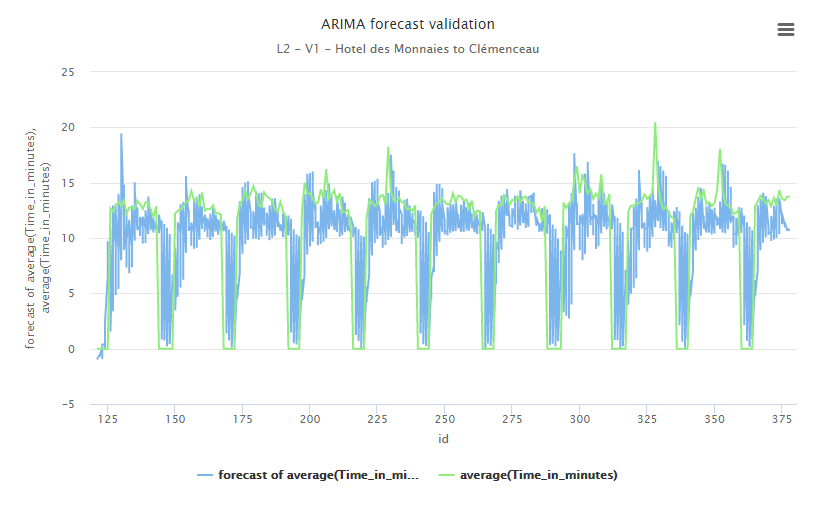
\includegraphics[width=\textwidth]{images/Fig6.png} 
    \caption{Forecast validation}
    \label{fig:valid}
\end{figure}

At last, the proposed model is used to forecast the travel time 3 hours after the end of the time series. Figure \ref{fig:ARIMA}, below, shows that the travel time should be decreasing. This proposition of the model is in line with intuition since the measurements were stopped at the end of a weekday.

 \begin{figure}[H]
    \centering
    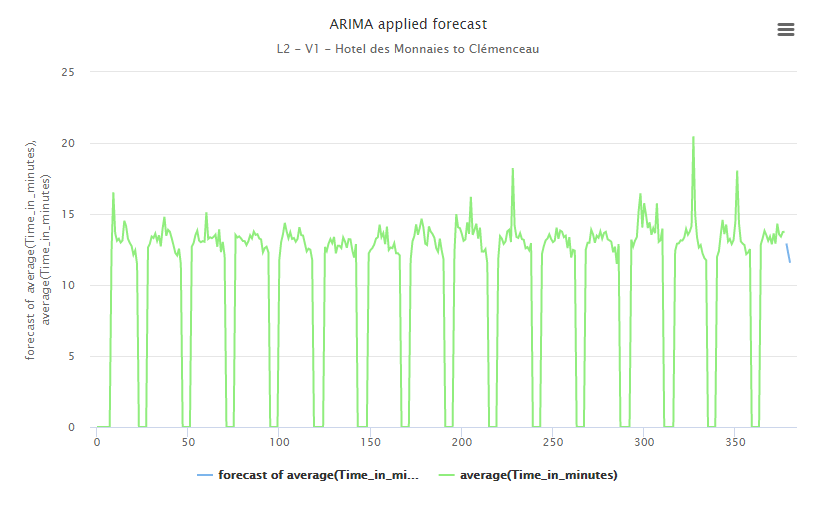
\includegraphics[width=\textwidth]{images/Fig7.png} 
    \caption{ARIMA forecast}
    \label{fig:ARIMA}
\end{figure}

\section{GPS tracks inference}
For this task of the project, a list of tracks is given, and it is requested the transport mode of these tracks is inferred. The tracks file is a simple \texttt{csv} file which contains several points for each track. Each point has the following data:
\begin{itemize}
     \item \texttt{TrackID}: An Integer indicating the track to which the point belongs.
     \item \texttt{lat} : A float which indicates the latitude of the point.
     \item \texttt{lon} : A float which indicates the longitude of the point.
     \item \texttt{time} : A string which indicates at which instant this data has been collected.
\end{itemize}

\subsection{Data processing}

The most challenging part of this task was to find an \textit{appropriate intersection} between these data and the data which was available from STIB. Finally, it has been decided to use both \textbf{position analysis} and \textbf{speed analysis} in order to indicate transport mode of a given track.

\subsubsection{Position analysis}
In order to find such a positional intersection, STIB \texttt{shape files} have been used. Several libraries of Python have been used to extract the points of each line. The library \textbf{GeoPandas} maybe was the most useful library that has been used. The STIB \texttt{shape files} contain feature dictionary or implement the \texttt{\_\_geo\_interface\_\_} of lines. This data has been extracted by using the \texttt{GeoDataFrame.from\_features} method. The following figures illustrate the data extraction that has been performed in this step:
\newline
\begin{figure}[htbp]
  \begin{minipage}[hb]{7cm}
    \centering
    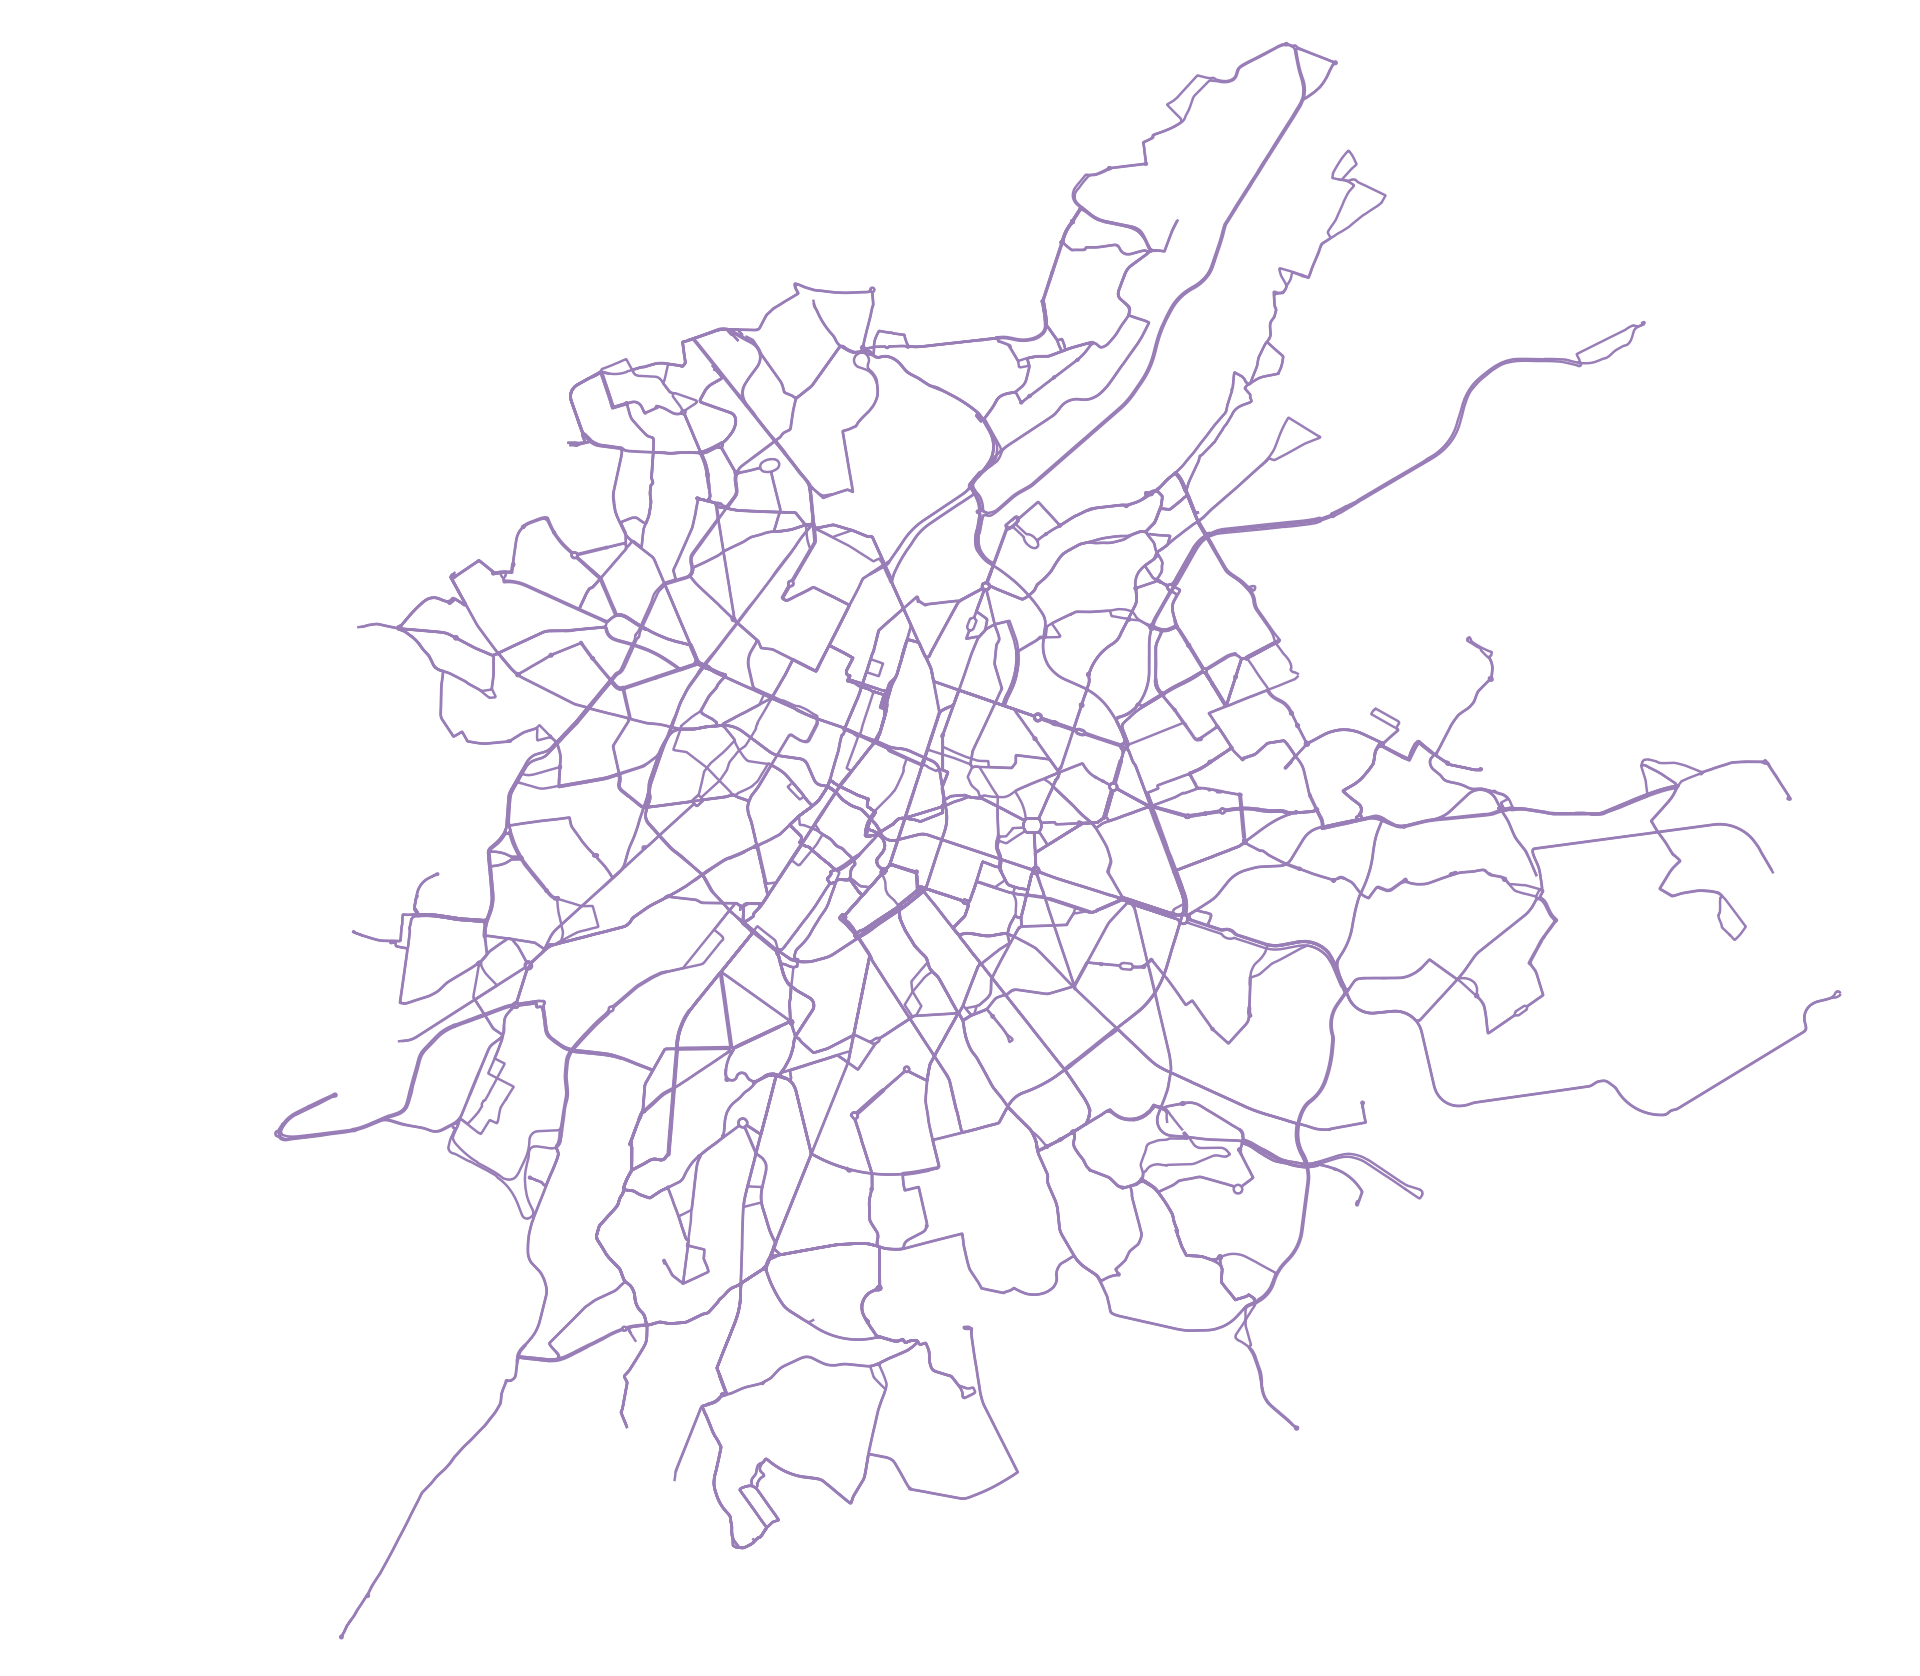
\includegraphics[width=\textwidth, height=6.65cm]{images/lines.png}
    \caption{STIB lines scheme}
  \end{minipage}
  \hspace{2cm}
  \begin{minipage}[hb]{7cm}
    \centering
    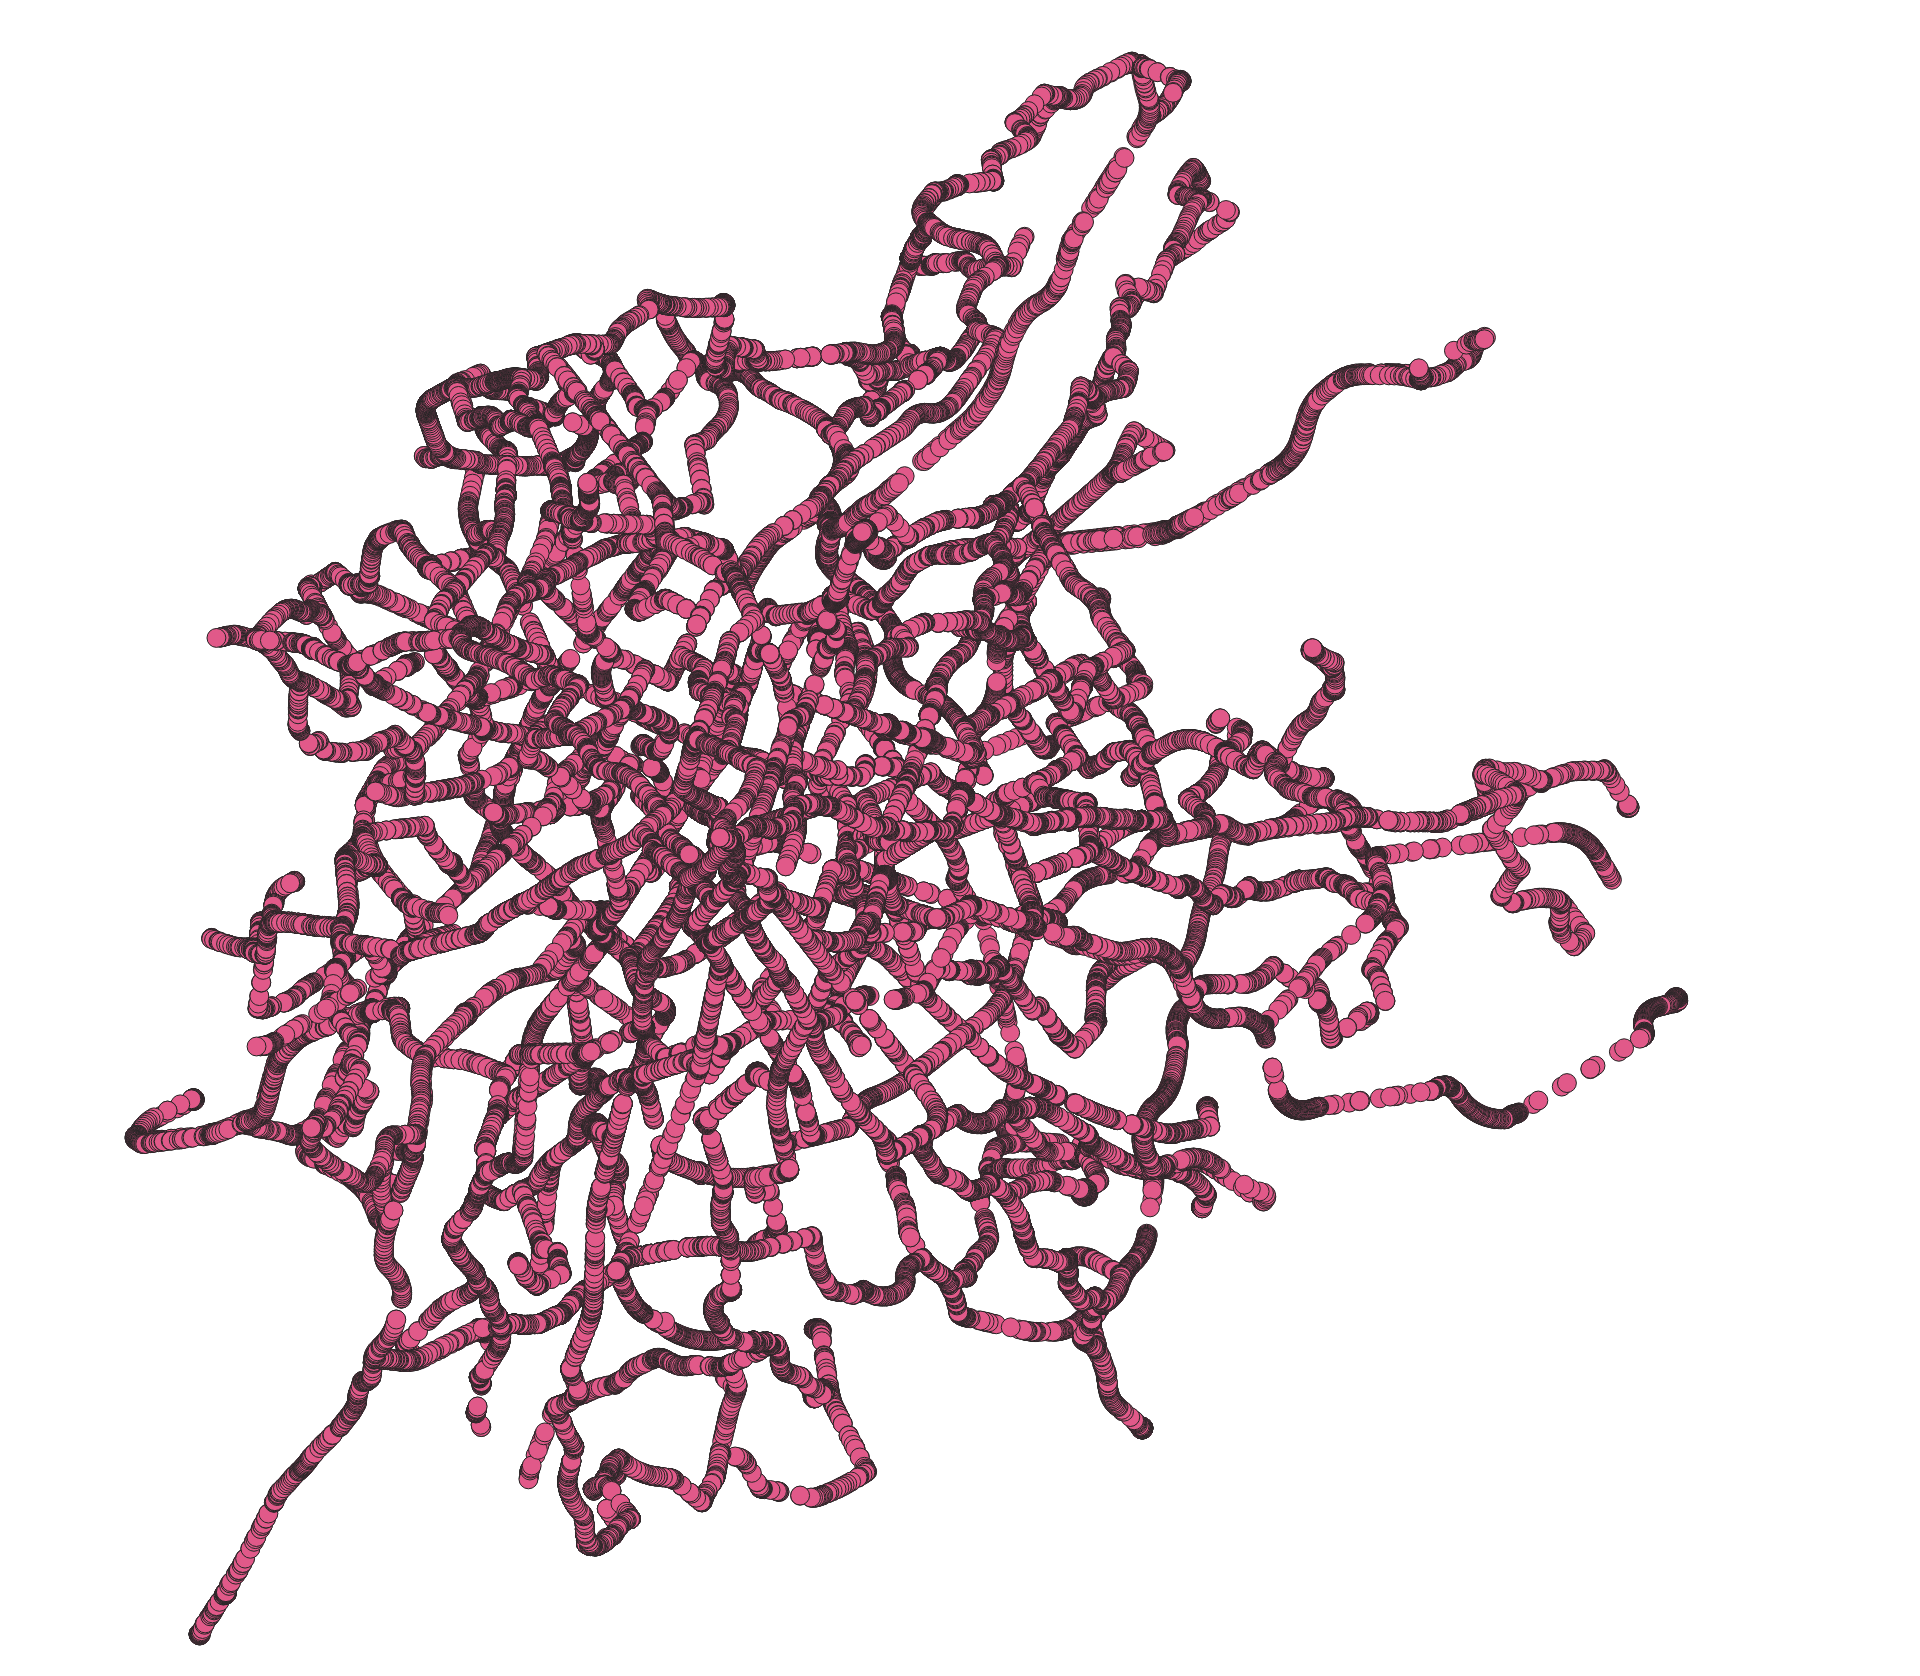
\includegraphics[width=\textwidth, height=6.65cm]{images/linesPoints.png}
    \caption{Points of STIB lines}
  \end{minipage}
\end{figure}
\newline
Once lines points have been extracted, the following process have been used:
\begin{enumerate}
    \item Each point of each track, $P_t$, has been compared with each point of each line, $P_l$ (line variant also have been taken into consideration). For this comparison, the challenging part was that $P_t$ and $P_l$ had different CRS (Coordinate Reference System). STIB data use the \textit{Belgian Lambert 72 (EPSG: 31370)} CRS while tracks CRS is \textit{WGS 84 (World Geodetic System) (EPSG: 4326)}. So the tracks points CRS have been set to \textit{Belge Lambert 72 (EPSG: 31300)} in order to be comparable with STIB lines points.
    \item If the distance between $P_t$ and $P_l$ was less than 10 meters, then the line $l$ is set to be a candidate for the point $P_t$.
    \item If the line $l$ was a candidate for at least $\frac{3}{4}$ of track points, it has been considered as a candidate line for that track.
    \item A list provided in order to contain all candidate lines.
\end{enumerate}
\subsubsection{Speed analysis}

Once candidate lines list is prepared, speed analysis is performed. The speed analysis is very important because in this step it becomes possible to identify if the traveller is in a STIB vehicle or he/she is using his/her own vehicle.
The following steps are implemented in order to analyze speed:
\begin{enumerate}
    \item For each candidate line, the closest stop to the first point of the track, $P_s$, and the last point of the track, $P_e$, is found.
    \item By using the analysis of the first task, the average speed between $P_s$ and $P_e$ is calculated.
    \item The average speed of the track is calculated. As each point of the track is provided almost instantly, a scale of 30 seconds is defined for this calculation. The reason of using this scale, is that the points that have been used in order to calculate average speed for the speed analysis task, has a time difference of almost 30 seconds.
    \item If, for a candidate line, the average speed of the track and the average speed that has been calculated by using the first task analysis, have a difference larger than 15 $\frac{km}{h}$, this candidate line is ignored. Otherwise, the candidate line is considered as the track line.
\end{enumerate}
It is noteworthy that, if more than one candidate line satisfies the conditions, the line with maximum number of points (position) correspondence has been considered as the track line.

\subsection{Results}
The result of execution using the file \texttt{GPStracks.csv} is shown below: 
\subsubsection{Track ID 1}
\begin{verbatim}
Track ID:   1
.........................
Position analysis: 

Candidate lines:  [] 
Votes:  []  /  178
Percentages:  []
.........................
Speed analysis: 

.........................
Result: 

Track:  1  --> transport mode Other (Probably the line is:  None )
\end{verbatim}
\subsubsection{Track ID 3}
\begin{verbatim}
Track ID:   3
.........................
Position analysis: 

Candidate lines:  [('032t', 1), ('032t', 2), ('082t', 1), ('082t', 2), ('049b', 2), ('050b', 2)] 
Votes:  [88, 91, 88, 91, 91, 91]  /  115
Percentages:  [76.522, 79.13, 76.522, 79.13, 79.13, 79.13]
.........................
Speed analysis: 

Line and variance  ('32', '1') 
Stops (from --> to):  0631  -->  5123
Average line speed:  0.0
Average track speed:  22.29658714734742
.........................
Line and variance  ('32', '2') 
Stops (from --> to):  0636  -->  5159F
Average line speed:  -inf
Average track speed:  22.29658714734742
.........................
Line and variance  ('82', '1') 
Stops (from --> to):  0631  -->  5123
Average line speed:  15.062294002987745
Average track speed:  22.29658714734742
.........................
Line and variance  ('82', '2') 
Stops (from --> to):  0636  -->  5159F
Average line speed:  -inf
Average track speed:  22.29658714734742
.........................
Line and variance  ('49', '2') 
Stops (from --> to):  2500  -->  5159
Average line speed:  -inf
Average track speed:  22.29658714734742
.........................
Line and variance  ('50', '2') 
Stops (from --> to):  2500  -->  5159
Average line speed:  -inf
Average track speed:  22.29658714734742
.........................
Result: 

Track:  3  --> transport mode t (Probably the line is:  82 )
\end{verbatim}
\subsubsection{Track ID 4}
\begin{verbatim}
Track ID:   4
.........................
Position analysis: 

Candidate lines:  [('050b', 2), ('050b', 1)] 
Votes:  [233, 211]  /  241
Percentages:  [96.68, 87.552]
.........................
Speed analysis: 

Line and variance  ('50', '2') 
Stops (from --> to):  5159  -->  2663
Average line speed:  -inf
Average track speed:  14.16390422669891
.........................
Line and variance  ('50', '1') 
Stops (from --> to):  2546  -->  5721
Average line speed:  15.765670238368289
Average track speed:  14.16390422669891
.........................
Result: 

Track:  4  --> transport mode b (Probably the line is:  50 )
\end{verbatim}
\subsubsection{Track ID 5}
\begin{verbatim}
Track ID:   5
.........................
Position analysis: 

Candidate lines:  [('032t', 1), ('032t', 2), ('082t', 1), ('082t', 2), ('097t', 1), ('097t', 2)] 
Votes:  [200, 198, 200, 198, 198, 193]  /  218
Percentages:  [91.743, 90.826, 91.743, 90.826, 90.826, 88.532]
.........................
Speed analysis: 

Line and variance  ('32', '1') 
Stops (from --> to):  2608F  -->  5123
Average line speed:  -inf
Average track speed:  15.9978424378629
.........................
Line and variance  ('32', '2') 
Stops (from --> to):  2663G  -->  5159F
Average line speed:  0.0
Average track speed:  15.9978424378629
.........................
Line and variance  ('82', '1') 
Stops (from --> to):  2608F  -->  5123
Average line speed:  -inf
Average track speed:  15.9978424378629
.........................
Line and variance  ('82', '2') 
Stops (from --> to):  2663G  -->  5159F
Average line speed:  14.998223517057735
Average track speed:  15.9978424378629
.........................
Line and variance  ('97', '1') 
Stops (from --> to):  2608F  -->  5123
Average line speed:  -inf
Average track speed:  15.9978424378629
.........................
Line and variance  ('97', '2') 
Stops (from --> to):  2663G  -->  5175
Average line speed:  14.435552062173322
Average track speed:  15.9978424378629
.........................
Result: 

Track:  5  --> transport mode t (Probably the line is:  82 )
\end{verbatim}
\subsubsection{Track ID 6}
\begin{verbatim}
Track ID:   6
.........................
Position analysis: 

Candidate lines:  [] 
Votes:  []  /  277
Percentages:  []
.........................
Speed analysis: 

.........................
Result: 

Track:  6  --> transport mode Other (Probably the line is:  None )
\end{verbatim}
\subsubsection{Track ID 7}
\begin{verbatim}
Track ID:   7
.........................
Position analysis: 

Candidate lines:  [('007t', 1), ('007t', 2), ('025t', 1), ('025t', 2)] 
Votes:  [166, 189, 152, 175]  /  195
Percentages:  [85.128, 96.923, 77.949, 89.744]
.........................
Speed analysis: 

Line and variance  ('7', '1') 
Stops (from --> to):  0906  -->  5258
Average line speed:  -inf
Average track speed:  19.948385691111582
.........................
Line and variance  ('7', '2') 
Stops (from --> to):  0901  -->  3481
Average line speed:  13.851716761672703
Average track speed:  19.948385691111582
.........................
Line and variance  ('25', '1') 
Stops (from --> to):  0906  -->  3480
Average line speed:  -inf
Average track speed:  19.948385691111582
.........................
Line and variance  ('25', '2') 
Stops (from --> to):  0901  -->  2397F
Average line speed:  12.965666453178818
Average track speed:  19.948385691111582
.........................
Result: 

Track:  7  --> transport mode t (Probably the line is:  7 )
\end{verbatim}
\subsubsection{Track ID 8}
\begin{verbatim}
Track ID:   8
.........................
Position analysis: 

Candidate lines:  [] 
Votes:  []  /  314
Percentages:  []
.........................
Speed analysis: 

.........................
Result: 

Track:  8  --> transport mode Other (Probably the line is:  None )
\end{verbatim}
\subsubsection{Track ID 10}
\begin{verbatim}
Track ID:   10
.........................
Position analysis: 

Candidate lines:  [] 
Votes:  []  /  62
Percentages:  []
.........................
Speed analysis: 

.........................
Result: 

Track:  10  --> transport mode Other (Probably the line is:  None )
\end{verbatim}
\subsubsection{Track ID 11}
\begin{verbatim}
Track ID:   11
.........................
Position analysis: 

Candidate lines:  [('025t', 1)] 
Votes:  [179]  /  209
Percentages:  [85.646]
.........................
Speed analysis: 

Line and variance  ('25', '1') 
Stops (from --> to):  5462F  -->  0906
Average line speed:  14.898977287950377
Average track speed:  26.457712832170717
.........................
Result: 

Track:  11  --> transport mode t (Probably the line is:  25 )
\end{verbatim}

\subsubsection{GPStracks analysis in one sight}

The following table shows the result of execution for file \texttt{GPStracks.csv}:
\begin{center}
    \begin{tabular}{ | c | c | c | c | c | c | }
        \hline
        Tracks ID/ Information & Transport mode & Possible line  \\ \hline
        1  & Other (o) & ---  \\ \hline
        3  & Tram (t) & 82  \\ \hline
        4  & Bus (b) & 50  \\ \hline
        5  & Tram (t) & 82  \\ \hline
        6  & Other (o) & ---  \\ \hline
        7  & Tram (t) & 7  \\ \hline
        8  & Other (o) & ---  \\ \hline
        10 & Other (o) & ---  \\ \hline
        11 & Tram (t) & 25  \\ \hline
    \end{tabular}
\end{center}


%\section{Personal analysis}
\section{Reachability analysis}
Another useful analysis to perform on this data is the reachability. Given a point in the map and a time interval, the algorithm gives as set of places where this point is reachable within the time limit. It can also be seen the other way around, it gives the set of places that are reachable from the point within the time limit. This information can be used by the police (or \texttt{STIB} security) to catch a fugitive, it would allow us to set perimeters around the different places the person could have reached.

\subsection{Data processing}
Due to the limitations of the data availability, It was decided to take into account only the following means of locomotion:

\begin{itemize}
    \item The different public transports of STIB
    \item Walking, assumed to be $5 \frac{km}{h}$
\end{itemize}

\subsubsection{Algorithm}

The algorithm works in an iterative mode.

The first step is to list all the stop ID that are reachable by running within the time interval from the point, as well as the theoretical arrival time.

Next, the iteration phase begins.

For each stop that just got added or modified at the last iteration, all the stops which are reachable within the time left are listed. These reachable stops are either obtained by walking or by taking transports. Next, these stops are merged with the main list of stops such as if a stop is already present in the main list, the arrival time is checked, if this arrival time is earlier than the one of the main list, it is modified with the current one, else it is dismissed.

The iteration stops when there are no longer any new or modified stops in the main list.



\subsection{Result}

The results below were obtained by giving the start position located in the middle of the ULB's campus Solbosch at the $23^{rd}$ October 2021, at 08:10 and 23:10, respectively.


\begin{figure}[H]%
    \centering
    \subfloat[\centering 08:10]{{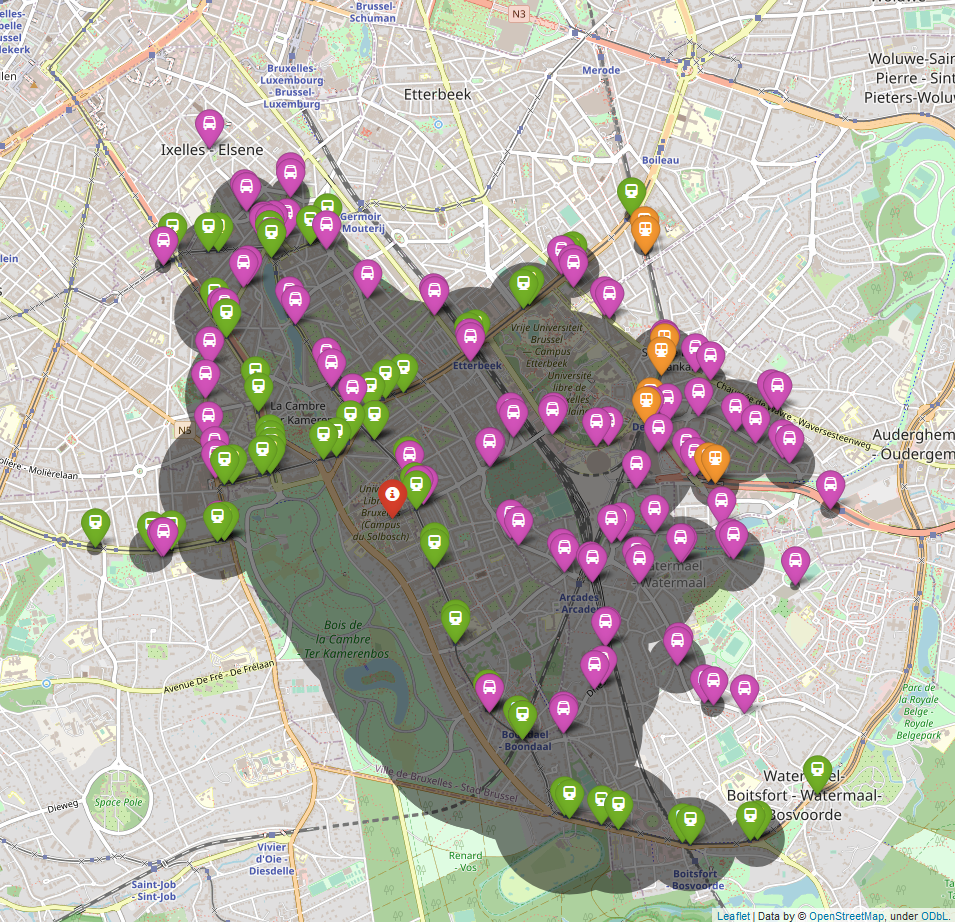
\includegraphics[width=7.75cm]{images/Task5Morning.png}  }}%
    \qquad
    \subfloat[\centering 23:10]{{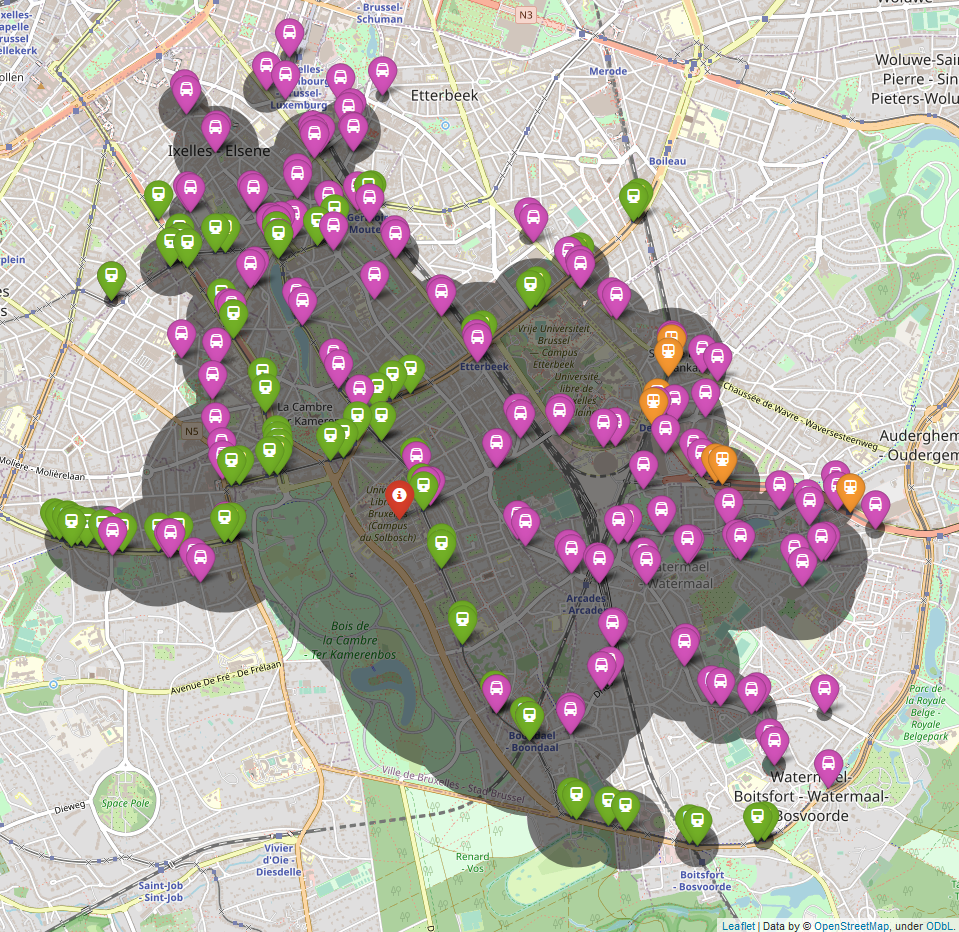
\includegraphics[width=7.75cm]{images/Task5Night.png} }}%
    \caption{Reachable places with 15 minutes from ULB at 23/10/2021}%
\end{figure}

In these results, it can be seen that in the morning the reachable area is more expanded than the one at night. This can easily be explained, as the average speed at 23h is higher than at 8h. It can also be seen that the area in the morning is not totally included in the one at night. It can be due to certain lines having their speed evolves differently in time. Another reason could be simply a problem in the data, such as missing or too few data.


\section{Conclusion}

Data preparation was certainly the biggest challenge for this project. In particular, the algorithm that creates the vehicle IDs based on the vehicle positions available in the \texttt{JSON} file has a great influence on the results. Any mistake in this algorithm may have severe repercussions on the results of all following tasks.

Considering the consistent results (speeds, delays, etc. for the 3 transport modes) exposed in this report, the way this data preparation was done by our team is considered sufficient to obtain interesting results as shown in this report, but could be improved if a vehicle ID was provided in the input data.

In addition to this major drawback, some corrections could be brought to the data, such as:
\begin{itemize}
    \item Adding the trip id's to all vehicle positions. This would be really helpful to compute the time delays more precisely.
    \item Adding the metros positions with regard to last stop would be helpful to have a more detailed analysis of metros speed, just like for buses and tramways.
    \item Harmonising the Stop IDs between the \texttt{JSON} files and the \texttt{GTFS} files would make the analysis more straightforward (currently some are different between the two databases).
    \item Etc.
\end{itemize}

Despite these minor issues, it is very interesting to observe how a public company like STIB / MIVB shares some of its information publicly. The possibilities that this decision has opened are infinite and we believe that this can only contribute to the development of deeper knowledge of Brussels' public transports and to the development of tools to improve users' experience and, eventually, to make their trips faster and safer.

\newpage

\appendix

\section{User manual}

In order to reproduce the results presented in this report, the following steps should be taken.

\subsection{Prerequisite}

\subsubsection{Directory disposition}
For all the scripts and processes to work as expected, the necessary files should be placed as follows: 

\dirtree{%
.1 \myfolder{red}{Root}.
.2 \myfolder{blue}{Data}.
.3 \myfolder{blue}{gtfs3Sept}.
.4 \myfolder{green}{...}.
.3 \myfolder{blue}{gtfs23Sept}.
.4 \myfolder{green}{...}.
.3 \myfolder{blue}{CSV}.
.3 \myfolder{blue}{JSON}.
.4 \myfolder{green}{vehiclePosition01.json}.
.4 \myfolder{green}{...}.
.4 \myfolder{green}{vehiclePosition13.json}.
.3 \myfolder{green}{shapefiles23Sept.zip}.
.3 \myfolder{green}{LinesInformation.csv}.
.3 \myfolder{green}{GPStracks.csv}.
.2 \myfolder{blue}{Processes}.
.3 \myfolder{green}{Task1.rmp}.
.3 \myfolder{green}{Task1\_2.rmp}.
.3 \myfolder{green}{Task2.rmp}.
.3 \myfolder{green}{Task3.rmp}.
.2 \myfolder{blue}{Scripts}.
.3 \myfolder{green}{JSONToCSV.py}.
.3 \myfolder{green}{Main.py}.
.3 \myfolder{green}{ExtractData.py}.
.3 \myfolder{green}{calendar\_handler.py}.
.3 \myfolder{green}{Analyze.py}.
.3 \myfolder{green}{Transport.py}.
.3 \myfolder{green}{Task4.py}.
.3 \myfolder{green}{Task5.py}.
}

The directories are represented in blue and the files in green.


\subsubsection{Software}
Python 3 (3.9.7) should be installed as well as several libraries listed below:
    
    \begin{itemize}
        \item Geopandas (0.9.0)
        \item Folium (0.12.1.post1)
        \item Haversine (2.5.1)
    \end{itemize}

The libraries themselves have dependencies, which is not a problem, as \texttt{pip} should automatically install them.

\subsubsection{Data generation}

Several files need to be generated in order to be able to launch the different tasks.

These python scripts should be executed in the \texttt{Scripts} directory:

\begin{lstlisting}
    $ python3 JSONToCSV.py
    $ python3 Main.py
\end{lstlisting}

Then, another files have to be generate by running the \texttt{Task1} process on RapidMiner.



\subsection{Task 1}

The task is entirely processed in RapidMiner.

As the task is a prerequisite of several tasks, all the needed files have already been generated. To visualize the results, it is simply needed to execute the task1\_2 process.


\subsection{Task 2}

First this line should be run:

\begin{lstlisting}
    $ python3 calendar_handler.py
\end{lstlisting}

Then the task is entirely processed in RapidMiner. The file \texttt{task2.rmp} should be imported and executed.


\subsection{Task 3}

This task is entirely processed in RapidMiner. The input file is \texttt{vehiclePositionID.csv}. In order to run the process, the file \texttt{task3.rmp} should be first imported in RapidMiner.

Then, boxes \texttt{START STOP} and \texttt{END STOP} should be filled in with the \texttt{LineID}, \texttt{Variance} and \texttt{PointIDs} for the start and end stop.

Based on this input, the data exploration subprocess will highlight the appropriate p and q parameters to use for the ARIMA forecasting model.

The other variable to choose in the applied ARIMA forecasting, is the forecast horizon (number of values to forecast).

The ARIMA forecast validation and the applied ARIMA model will run in a second step in order to calculate and show the final result of forecasting.



\subsection{Task 4}

In order to run the algorithm of the GPS tracks inference, it is simply needed to execute the \texttt{Task4.py} file with Python 3.

By default, only the provided tracks are loaded and analyzed. To analyze other tracks, it is simply needed to change the path of the file passed in the \texttt{readTracks} function.


\subsection{Task 5}

In order to run the algorithm of the reachability analysis, it is simply needed to execute the \texttt{Task5.py} file with Python 3.

To change different parameters, it is just needed to modify the values in the main function. By default, these values are set to the one used in the report at the result section of the reachability analysis.



\end{document}
